\documentclass[journal,twoside,web]{ieeecolor}
\usepackage{generic}
\pdfminorversion=4

\let\proof\relax
\let\endproof\relax
\usepackage{amsthm}
\usepackage{graphicx}
\usepackage{epsfig}
\usepackage{times}
\usepackage{amsmath}
\usepackage{amssymb}
\usepackage{cleveref}
\usepackage{subcaption,graphicx}
\usepackage{mathtools, cuted}
\usepackage{todonotes}
\usepackage{url}
\usepackage{xcolor}
\usepackage{mathrsfs}
\usepackage{multirow}
\usepackage{caption}
\usepackage{subcaption}
\usepackage{cite}
\usepackage{wrapfig}
\usepackage{float}
\usepackage{mleftright}
\usepackage{nth}
\usepackage{dsfont}
\usepackage[normalem]{ulem}
\usepackage{tikz}
\usetikzlibrary{shapes,arrows}
\usepackage{booktabs}

% Define revision color for IEEE class compatibility
\definecolor{revisionblue}{rgb}{0,0,0.8}
\definecolor{reviewerred}{rgb}{0.8,0,0}
\definecolor{oldgray}{rgb}{0.5,0.5,0.5}
% Command for marking revisions
\newcommand{\rev}[1]{\textcolor{revisionblue}{#1}}
% Command for reviewer comment annotations
\newcommand{\revnote}[1]{\textcolor{reviewerred}{\textit{#1}}}
% Command for old text that was removed/replaced
\newcommand{\old}[1]{\textcolor{oldgray}{\sout{#1}}}

\newtheorem{theorem}{Theorem}
\newtheorem{acknowledgement}[theorem]{Acknowledgement}
\newtheorem{algorithm}[theorem]{Algorithm}
\newtheorem{axiom}[theorem]{Axiom}
\newtheorem{assumption}[theorem]{Assumption}
\newtheorem{properties}[theorem]{Properties}
\newtheorem{case}[theorem]{Case}
\newtheorem{claim}[theorem]{Claim}
\newtheorem{conclusion}[theorem]{Conclusion}
\newtheorem{condition}[theorem]{Condition}
\newtheorem{conjecture}[theorem]{Conjecture}
\newtheorem{corollary}{Corollary}
\newtheorem{criterion}[theorem]{Criterion}
\newtheorem{con}[theorem]{Condition}
\newtheorem{definition}{Definition}
\newtheorem{exercise}[theorem]{Exercise}
\newtheorem{lemma}{Lemma}
\newtheorem{notation}[theorem]{Notation}
\newtheorem{problem}[theorem]{Problem}
\newtheorem{proposition}[theorem]{Proposition}
\newtheorem{solution}[theorem]{Solution}
\newtheorem{summary}[theorem]{Summary}
\newtheorem{remark}{Remark}
\newtheorem{example}[theorem]{Example}
\newtheorem{thm}{Theorem}
\newtheorem{cor}{Corollary}
\newtheorem{lem}{Lemma}
\newtheorem{prop}{Proposition}
\newtheorem{defn}{Definition}
\newtheorem{rem}{Remark}
\newtheorem{ass}{Assumption}

\DeclareMathOperator*{\infm}{inf}
\DeclareMathOperator*{\minimize}{minimize}
\DeclareMathOperator*{\maximize}{maximize}
\DeclareMathOperator*{\subjt}{subject \ to}
\DeclareMathOperator*{\sgn}{sign}
\DeclareMathOperator*{\argmin}{argmin}
\newcommand{\argmax}[1]{\underset{#1}{\operatorname{arg}\,\operatorname{max}}\;}
\newcommand{\pe}{\psi}
\newcommand{\R}{\mathbb{R}}
\newcommand{\trace}{\text{tr}}
\newcommand{\vecu}{{\bf u}}
\newcommand{\vece}{{\bf e}}
\newcommand{\vecc}{{\bf c}}
\newcommand{\dom}{\mathcal{D}}
\newcommand{\op}{\mathcal{L}}
\newcommand{\dop}{\mathcal{E}}
\newcommand{\x}{\textbf{x}}
\newcommand{\z}{\mathbb{Z}}
\newcommand{\real}{\mathbb{R}}
\newcommand{\p}{\partial}
\newcommand{\ps}{p^{\star}}
\newcommand{\PF}{\mathbb{P}}
\newcommand{\Tyx}{T_{y\rightarrow x}(p)}
\newcommand{\bi}{\begin{itemize}}
\newcommand{\ei}{\end{itemize}}
\newcommand{\bd}{\begin{displaymath}}
\newcommand{\ed}{\end{displaymath}}
\newcommand{\be}{\begin{align*}}
\newcommand{\ee}{\end{align*}}
\newcommand{\si}{\Sigma^{-1}}
\newcommand\norm[1]{\left\lVert#1\right\rVert}
\newcommand{\sub}[2]{(#1)_{(#2)}}

\title{\LARGE \bf Robust Optimization via Continuous-Time Dynamics}

\author{Keivan Ebrahimi, Nicola Elia, and Umesh Vaidya\\
\thanks{Financial support from the National Science Foundation grants CNS-1329915, ECCS-1150405, CIF-1220643, and ECCS-1810079 and from AFOSR grant FA95500119 are gratefully acknowledged. K. Ebrahimi is with the Department of Electrical \& Computer Engineering, Iowa State University, Ames, Iowa. U. Vaidya is with the Department of Mechanical Engineering, Clemson University, Clemson SC.  N. Elia is with the Department of Electrical and Computer Engineering, University of Minnesota, Twin Cities.
{\tt\small keivan@iastate.edu},
{\tt\small uvaidya@clemson.edu},
{\tt\small nelia@umn.edu}
}}

\begin{document}

\pagestyle{headings}
\setcounter{page}{1}
\pagenumbering{arabic}

\maketitle

\begin{abstract}
\rev{Robust optimization problems arise in numerous applications where system parameters are uncertain but bounded within known sets. Traditional solution methods require either explicit robust counterpart reformulations, which are often intractable, or scenario-based sampling approaches that scale poorly with problem dimension. This paper introduces RO dynamics—a continuous-time dynamical system that directly solves min-max robust optimization problems without requiring reformulations or uncertainty model specifications. Our key contributions establish the saddle point property without joint convexity-concavity and construct a novel Lyapunov function proving global convergence for general convex-concave problems. The method operates using only output feedback, enabling model-free operation and decentralized implementation in real-time applications. Numerical experiments demonstrate speedup over scenario sampling methods, with exact solutions for robust quadratic programming with ellipsoidal uncertainties, nonlinear optimization where robust counterparts cannot be derived, and distributed sensor placement. These results establish continuous-time dynamics as a powerful alternative paradigm for robust optimization, particularly suited for online adaptation and physical system implementation.}
\end{abstract}

\section{Introduction}

\rev{Optimization problems in engineering, finance, and machine learning often involve uncertain parameters that must be handled robustly to ensure reliable performance.} Two different approaches can be used: stochastic optimization, where uncertainty is treated as a random variable, or RO, where uncertainty is assumed to be deterministic and bounded. Unlike stochastic optimization, RO does not require any known probability distributions in the problem data. Instead, RO assumes that the uncertain data reside within a predefined uncertainty set, for which constraint violation cannot be tolerated. For more information on robust and stochastic optimization-based approaches, see \cite{bental2009}, \cite{bertsimas2011}, and the references therein. Early works on RO include \cite{soyster1976}, which considered robust linear optimization with ellipsoidal uncertainty sets, and \cite{falk1976}, which presented exact solutions of inexact linear programs as a simple case of RO.

The problem of robust linear programming was studied in \cite{bental1999}, while robust conic-quadratic optimization and robust semi-definite optimization were discussed in \cite{bental2002} and \cite{bental1998}, respectively. Refer to \cite{bertsimas2011} and \cite{beyer2007} for \rev{comprehensive} surveys of RO problem solutions.

\rev{Recent developments in distributionally robust optimization (DRO) have bridged the gap between stochastic and robust approaches \cite{aigner2023,yang2023}.}

\cite{xu2009} and \cite{xu2010} showed that machine learning algorithms such as the norm-regularized support vector machine and the Lasso problem could be interpreted as RO problems. \rev{Recent work has further integrated robust optimization with machine learning \cite{zhu2023zeroth,madry2018adversarial}.}

One of the main standard approaches for solving RO problems involves constructing a robust counterpart (RC) equivalent to the RO problem \cite{bental2009}. This widely used method essentially tries to find a deterministic equivalent to RO problem through a reformulation. In this sense, the practicality of robust programming depends on whether or not its RC is computationally tractable. An overview of different RO problems with tractable conjugates can be found in \cite{gorissen20152} Table 1 for some of which RC cannot be found.
The reformulation approach to solving the RO problem, which is often a challenging, albeit usually convex, optimization problem, has the deficiency of suffering from case-by-case scenarios depending on the specific form of the uncertainty constraint and the specific form of the uncertainty set. In other words, depending on how simple the uncertainty set looks and based on the optimization problem type (whether it is linear programming, quadratic programming, second-order cone programming, semi-definite programming, etc.), an RC is being calculated and provided at hand. These reformulations may be computationally more expensive than other approaches \cite{bertsimas2016}. Hence, the absence of a unified framework for solving a general class of RO problems without prior knowledge of the problem formulation is strongly felt.

By calculating a concave conjugate of nonlinear constraint functions and supporting the function of uncertainty sets, \cite{bental20152} and \cite{gorissen20152} used the Fenchel duality to obtain a tractable RC for new classes of robust nonlinear optimization (RNO) problems. However, when no closed form is available for the convex conjugate function of an uncertainty set or convex/concave conjugates of a non-linear constraint, these approaches still cannot obtain the RC for many sets of nonlinear uncertainties and constraints. \rev{Moreover, all these methods require either explicit problem structure knowledge or extensive computational resources, unlike our dynamics-based approach.}

An alternative randomized approach based on constraint sampling is an approximate probabilistic relaxation solution to RO problems as seen in \cite{calafiore2004} and \cite{calafiore2010} where a finite set of high-dimensional deterministic optimization problems obtained from sampling are solved. This approach does not require concavity of the constraint in the uncertain variable but due to the large number of required scenarios to approximate the stochasticity of these problems, the stochastic optimization involves formulating a large-scale scenario program, which is in general computationally demanding.
\rev{Recent methods include ADMM decomposition \cite{rostampour2021}, achieving improved convergence rates for distributed robust optimization problems.}

In another effort, \cite{bental2015} incorporated the min-max behavior of RO problems to solve them by an oracle-based approximate robust optimization algorithm based on oracle-based subgradient descent and interior point methods. The proposed algorithms find an approximate robust solution using a number of calls to an oracle that solves the original (non-robust) problem. However, the solution would be approximated with some predetermined accuracy, $\eta$, with the number of iterations growing to $\mathcal{O}(\frac{1}{\eta})$, as the algorithm approximates the RC by invoking the Oracle a polynomial number of times.
\rev{Classical cutting-plane approaches \cite{mutapcic2009} treat RO problems as semi-infinite programming but have limitations when pessimization oracles are approximate.} In another effort, \rev{Robust optimization over time (ROOT) combines robust optimization with dynamic optimization \cite{yazdani2023,aigner2023}.}

In this paper, we provide the architecture of a dynamical system that converges to the optimal robust solution for a large class of RO problems. Our approach builds on classical primal-dual systems \cite{arrow1958,feijer2010} but addresses the unique challenges posed by the min-max structure of robust optimization.

\rev{\textbf{Main Contributions:} The contributions of this paper are as follows:}
\begin{enumerate}
\item \rev{\textbf{Model-free operation:} We develop a continuous-time dynamical system that solves RO problems using only output feedback, without requiring explicit knowledge of uncertainty models or problem structure. This enables implementation in physical systems where only measurements are available.}

\item \rev{\textbf{Unified framework:} Our method provides a single dynamical system architecture that handles all convex-concave RO problems uniformly, eliminating the need for problem-specific reformulations or case-by-case analysis required by robust counterpart methods.}

\item \rev{\textbf{Novel saddle point theory:} We prove that the saddle point property holds for RO problems despite the Lagrangian lacking joint convexity-concavity—a fundamental violation of standard theory. This theoretical achievement (see Section \ref{section_saddle}) enables the application of dynamical methods to robust optimization.}

\item \rev{\textbf{Custom Lyapunov analysis:} We construct a non-standard Lyapunov function that establishes global asymptotic stability of the equilibrium corresponding to the robust optimal solution. The Lyapunov function design handles the complex interaction between primal, dual, and uncertainty variables.}

\item \rev{\textbf{Real-time adaptation:} The continuous-time nature of our approach enables real-time tracking of time-varying uncertainties and online adaptation, making it suitable for dynamic environments and decentralized implementation.}

\item \rev{\textbf{Broader problem scope:} Our method provides exact solutions for problems where robust counterparts are unknown or computationally intractable, including nonlinear constraints with complex uncertainty sets.}
\end{enumerate}

{\color{revisionblue}These contributions establish continuous-time dynamics as a powerful alternative paradigm for robust optimization, complementing existing discrete algorithmic approaches.} The proposed continuous-time optimization system can solve a general class of $\mathcal{RO}$ problems where the cost function and the constraints are convex (concave) with respect to the decision variables (uncertain variables) and the uncertainty sets are convex\footnote{Preliminary convergence results for a special formulation appeared without proofs in \cite{ebrahimi2019continuous}. In this paper, we generalize the problem formulation and provide complete proofs, which are the core of our contributions.}. This class includes all the cases in \cite[~Table 1]{gorissen20152}.


The remainder of this paper is organized as follows. In Section \ref{sec_RO}, we present the problem statement of $\mathcal{RO}$ in a slightly generalized form. In Section \ref{section_saddle}, the characterization of saddle property and KKT optimality conditions along with the Lagrangian function for $\mathcal{RO}$ problem are provided. The main results on how to construct the $\mathcal{RO}$ dynamics is presented in Section \ref{section_pddynamics}. This section also includes the Lyapunov-based global convergence result. We then present simulation results in Section \ref{section_simulations} followed by conclusions in Section \ref{section_conclusions}.
Finally, detailed proofs are mentioned in the Appendix.

\section{Notations}\label{notations}

We define $i=0,\cdots,N$ as $i\in[N]$, and $i=1,\cdots,N$ as $i\in[N]^+$. In addition, $\left[\cdot\right]_\eta^+$ shows the positive projection defined as follows for the scalar-valued function $P$
\begin{align} \label{proj}
[P]_\eta^+:=\left\{\begin{array}{ccl}P&{\rm if}& P>0 \;{\rm or} \;\eta>0\\
0&{\rm otherwise}
\end{array}\right..
\end{align}
For vector-valued $P$, the projection is defined element-wise.

\section{Robust Optimization Problems}\label{sec_RO}
Given an objective $f_0(x)$ to optimize, subject to constraints $f_i(x,u_i) \leq 0$ with uncertain parameters, $\{u_i\}$, a classical robust optimization problem has the following form
$$
\begin{array}{ccc}
\mu&:=&\underset{x}{\min}\; f_0(x)\\
&&\text{s.t.}\;\;\;f_i(x,u_i)\leq 0,\;\;\;\; \forall \,u_i\in \mathcal{U}_i,\;\;\;i^+_{[N]}.
\end{array}
$$
where $x\in \real^n$ is a vector of decision variables, $f_0$ and $f_i$ are $\real^n \to \real$ functions, and the uncertainty parameters $u_i \in \real^{m_i}$ are assumed to take arbitrary values in certain convex compact uncertainty sets $\mathcal{U}_i \subseteq \real^{m_i}$.
The above problem is typically a semi-infinite optimization due to the cardinality of the $\mathcal{U}_i$. However, each robust constraint can be rewritten as a maximization problem as\footnote{\rev{Since the uncertainty set is compact and the constraint functions are continuous, the supremum is attained within the set; therefore, we can replace ``sup'' with ``max'' in our formulation.}}
\begin{align}
\begin{array}{ccc}
\mu&:=&\underset{x}{\min}\; f_0(x)\\
&&\text{s.t.}\;\;\;\displaystyle\max_{{u_i\in \mathcal{U}}_i} f_i(x,u_i)\leq 0,\;\;\;\;i^+_{[N]}
\end{array}\;.\label{standardRO}
\end{align}

We consider a slight variation of (\ref{standardRO}), which takes the following under the assumptions stated below.

\begin{equation}\label{RO0}
\mathcal{RO}_0\left\{ \begin{array}{ccc}
&\mu:=\underset{x}{\min} \;\underset{u_0\in \mathcal{U}_0}{\max}\; f_0(x,u_0)\\
&\text{s.t.}\;\;\;\underset{u_i\in \mathcal{U}_i}{\max}\;\; f_i(x,u_i)\leq 0\;,\;i\in[N]^+,\\ \\
&\mathcal{U}_i:=\{u_ i\in \mathbb{R}^{m_i}\;:\;h_{ij}(u_i)\leq 0,\;\;j\in[K_i]\}\;,\;i\in[N]
\end{array}\right.
\end{equation}
\rev{Here, $h_{ij}(u_i)$ represents the $j$-th constraint function defining the $i$-th uncertainty set $\mathcal{U}_i$, and $K_i$ denotes the total number of constraints that define $\mathcal{U}_i$.} 

\begin{remark}[\rev{Key Properties of Formulation (\ref{RO0})}]
\begin{enumerate}
\item \rev{\textbf{Generalization:} Formulation (\ref{RO0}) generalizes (\ref{standardRO}) by allowing uncertainty in the objective function and explicitly representing uncertainty sets via inequality constraints, facilitating the min-max-max-min structure essential for our dynamical approach.}
\item \rev{\textbf{Compactness:} Under the convexity assumptions stated below, uncertainty sets $\mathcal{U}_i$ remain compact since convex constraints preserve convexity and boundedness.}
\item \rev{\textbf{Nonlinear constraints:} Our framework handles nonlinear uncertainty constraints $h_{ij}(u_i) \leq 0$ through gradient terms $\nabla_{u_i} h_i(u_i)$ that naturally accommodate nonlinearity.}
\end{enumerate}
\end{remark}

The problem in (\ref{RO0}) reduces to the one in (\ref{standardRO}) when $\mathcal{U}_0$ is a singleton.
Following \cite{bental2009-2} and without loss of generality, we consider the $\mathcal{RO}$ problem dealing with constraint-wise uncertainties where each constraint $f_i$ is only a function of $u_i$.
The functions $f_i$ and $h_{ij}$ have scalar values with the following assumptions.

\begin{assumption}\label{assume1} The functions $h_{ij}(u_i)$ are convex in $u_i$ for $i\in[N]$ and $j\in[K_i]^+$.
The function $f_0(x,u_0)$ is strictly convex in $x$ for any $u_0\in \mathcal{U}_0$, and concave in $u_0$ for any $x$. Also, for $i^+_{[N]}$, $f_i(x,u_i)$ is convex in $x$ for fixed $u_i$ and concave in $u_i\in \mathcal{U}_i$, for fixed $x$.
Finally, the functions $f_i$ and $h_i$ $i\in[N]$ are $C^1$ with local Lipschitz gradients.
\end{assumption}

\begin{remark}[\rev{Justification of Assumption \ref{assume1}}]
\rev{The convex-concave structure ensures computational tractability and is satisfied by most practical $\mathcal{RO}$ problems.}
\end{remark}

\begin{assumption} \label{assume_feasible} Existence of optimal solutions and strong duality.

\begin{enumerate}
\item $\mathcal{RO}$ problem (\ref{RO}) is feasible. An optimal min-max solution $(x^\star,u^\star)$ exists and $\mu$ in the $\mathcal{RO}$ problem (\ref{RO}) is finite.
\item $\mathcal{RO}$ problem satisfies the Slater constraint qualification, for both the upper level optimization and the lower level maximization problems
 \cite{bental2009-2}, that is,
for all $i\in[N]$ and all $j\in[K_i]^+$, there exist $u_i \in \mathcal{U}_i$ such that $h_{ij}(u_i)<0,\;$  and
for $i^+_{[N]}$,  there exists $x \in \mathbb{R}^n$ such that, $\mathcal{F}_i(x)<0$\;.
\end{enumerate}
\end{assumption}
\begin{remark}
    It should be noted that the uncertainty is often parametrized affinely in $\mathcal{RO}$ problem; hence, the concavity property of the $f_i$ functions is automatically satisfied.
\end{remark}
\begin{remark}[\rev{Justification of Assumption \ref{assume_feasible}}] \label{strong_duality_rem}
\rev{The Slater constraint qualification guarantees that the $\mathcal{RO}$ problem enjoys strong duality for upper and lower level optimization problems \cite[Section~5.2.3, 5.9.1]{boyd2004}. While this assumption may appear restrictive, it can often be satisfied or relaxed in practice:}
\begin{enumerate}
\item \rev{In many robust optimization applications, the uncertainty sets are designed with strict feasibility in mind (e.g., ellipsoidal sets with positive radius).}
\item \rev{The assumption ensures that saddle point and optimal dual solutions exist \cite{bental2009-2}, which is crucial for our dynamical system approach.}
\item \rev{For cases where Slater conditions are too restrictive, alternative constraint qualifications such as those discussed in \cite{jeyakumar2010} can be employed.}
\item \rev{In practical implementations, the assumption can often be enforced by appropriate scaling or small perturbations of the constraint sets.}
\end{enumerate}
\end{remark}

Finally, we introduce the problem we consider in this paper, a slight generalization of $\mathcal{RO}_0$ in (\ref{RO0}).
\begin{equation}\mathcal{RO}\left\{\begin{array}{ccc}
&\mu:=\underset{x}{\min} \;\underset{u_0\in \mathcal{U}_0}{\max}\; f_0(x,u_0)+\displaystyle\sum_{i=1}^N c_i \underset{u_i\in \mathcal{U}_i}{\max}\;\; f_i(x,u_i)\label{RO}\\ \\
&\text{s.t.}\;\;\;\underset{u_i\in \mathcal{U}_i}{\max}\;\; f_i(x,u_i)\leq 0\;,\;i\in[N]^+,\\ \\
&\mathcal{U}_i:=\{u_ i\in \mathbb{R}^{m_i}\;:\;h_{ij}(u_i)\leq 0,\;\;j\in[K_i]\}\;,\;i\in[N]
\end{array}\right.
\end{equation}
where $c_i\geq 0$ for $i\in[N]^+$. This setting can be seen as an elementary regularized version of more common formulations $\mathcal{RO}_0$ obtained for $c_i=0$, $i\in[N]^+$.
The role of $c_i$ is further clarified below.

It is convenient to rewrite $\mathcal{RO}$ in the following form
\begin{align}
&\mu:=\underset{x}{\min} \; \mathcal{F}_0(x)+\sum_{i=1}^N c_i\mathcal{F}_i(x)\label{RO2}\\
&\;\;\text{s.t.}\;\;\;\mathcal{F}_i(x)\leq 0\;,\;i^+_{[N]}\;,\nonumber
\end{align}
where
\begin{equation}\label{G.eq}
\mathcal{F}_i(x):=\max_{u_i\in \mathcal{U}_i} f_i(x,u_i)\;,\; i\in[N]\;.
\end{equation}
In this paper, we often call (\ref{G.eq}) as the ``lower optimization problems'', and the minimization in (\ref{RO2}) as the ``upper optimization''.

\begin{remark}[\rev{Problem Formulation and $c_i$ Terms}]
\rev{Our formulation (\ref{RO}) adds regularization terms $c_i$ to the classical $\mathcal{RO}$ problem for three key reasons: (i) preventing singularity when constraints are inactive ($\lambda_i = 0$), (ii) improving numerical stability, (iii) recovering the classical problem as $c_i \to 0$. We maintain separate $c_i$ and $\lambda_i$ (rather than combined $\gamma_i$) to preserve dual variable interpretation and enable our Lyapunov construction.}
\end{remark}

As already mentioned, our formulation includes the typical robust optimization formulation $\mathcal{RO}_0$
\begin{equation}
\begin{array}{lcc}
\mu=&\;\displaystyle\min_x f_0(x)\\
s.t.&\; \mathcal{F}_i(x)\leq 0,\;\;i^+_{[N]}
\end{array}\;,
\label{RO3}
\end{equation}
or the form below that is popular in the machine learning context \cite{rafique2022,zhang2021}
\begin{equation}
\mu=\;\displaystyle\min_x\max_{u\in \mathcal{U}} f_0(x,u)\;.
\end{equation}
We finally introduce the following assumption valid for most of this paper.

\begin{assumption} \label{assume_c>0}
$c_i > 0$ for $i^+_{[N]}$.
\end{assumption}

\begin{remark}\label{active_inactive_constraint_rem} 
\rev{Assumption \ref{assume_c>0} provides regularization for inactive constraints. In practice, use small values (like $c_i = 10^{-6}$) for numerical stability. Section \ref{perturbed_section_pddynamics} analyzes the $c_i \to 0$ limit rigorously.}
\end{remark}

\subsection{Robust feasible solution and robust counterpart}
A meaningful solution to $\mathcal{RO}$ problem (\ref{RO}) has to be immune against the uncertainties in the sense that the solution vector $x$ should satisfy the constraints for all $u_i$'s within the uncertainty sets\footnote{Similar to what is meant by feasibility in Robust Control \cite{zhou1995}.}. Such vector $x$ is called a robust feasible solution (RFS). One approach to solving the problem (\ref{RO}) is to try to compute (\ref{G.eq}) in closed form.

For various important combinations of constraint functions $f_i$ and uncertainty sets $\mathcal{U}_i$, ($i>0$) it is possible to obtain an explicit convex function $\mathcal{F}_i$ \cite{bental2009}. A classical example is when $f_i$ is linear in $x$ for fixed $u_i$ and linear in $u_i$ for fixed $x$, while $\mathcal{U}_i$ is an ellipsoidal set.
Then, $\mathcal{F}_i$ can be easily derived as an explicit second-order conic function.
In this case, $\mathcal{RO}$ problem (\ref{RO}) becomes a nominal optimization problem (not affected by uncertainty) known as the explicit RC:
\begin{align} \label{rc}
\displaystyle \min_{\mathcal{F}_i(x)\leq 0} f_0(x)\;.
\end{align}
As shown in \cite{bental2009-2}, the RC is always a convex optimization problem under Assumption \ref{assume1}. While the RC is known for important classes of problems as described in \cite{bertsimas2011}, this approach requires problem-specific derivations; moreover, RC is generally difficult to find (See Section \ref{section_simulations} for an example). Instead, our proposed approach has a dynamical system that simultaneously finds the best RFS and the worst parameters $u_i$' s, independently of the specifics of the constraint functions and the uncertainty sets.


\section{Duality, KKT conditions and saddle property} \label{section_saddle}
The basic idea of this paper is to combine the usually separated and nested optimization (\ref{RO2}) and (\ref{G.eq}) into one Lagrangian optimization.

To derive the Lagrangian function for $\mathcal{RO}$ problem (\ref{RO}), we introduce Lagrange multipliers $\lambda_i\geq 0$ for $i^+_{[N]}$, and let $\lambda=(\lambda_1,\lambda_2,\cdots,\lambda_N)^\top \in \mathbb{R}_+^N$ where the non-negative orthant of $\mathbb{R}^N$ is denoted by $\mathbb{R}_+^N$. Note that $\mu$ in $\mathcal{RO}$ problem (\ref{RO}) can be written in short-hand notation  as follows
\begin{align}
\mu=&\;\underset{x}{\min}\;\underset{\lambda\geq 0}{\max}\; \mathcal{F}_0(x)+\sum_{i=1}^N (c_i+\lambda_i) \; \mathcal{F}_i(x)\;,
 \label{upper_ro}
\end{align}
where $\mathcal{F}_i(x)$ is given by (\ref{G.eq}).
 By introducing Lagrange multipliers $v_{ij} \geq 0$ for the maximization problem in (\ref{G.eq}) and defining
\begin{align*}
v_i:=(v_{i1},\cdots, v_{iK_i})^\top \in \mathbb{R}_+^{K_i},\;h_i:=(h_{i1},\cdots, h_{iK_i})^\top\;,\nonumber
\end{align*}
the lower level strong duality (according to Assumption \ref{assume_feasible}) yields
\begin{align} \label{lower_ro}
\mathcal{F}_i(x)=\underset{u_i\in \mathbb{R}^{m_i}}{\max}\;\underset{v_{i}\geq 0}{\min}\;f_i(x,u_i)-v_i^\top h_{i}(u_i)\;.
\end{align}

Defining the Lagrangian $\tilde{\mathcal{L}}_i:\mathbb{R}^n \times \mathbb{R}^{m_i} \times \mathbb{R}^{K_i} \rightarrow \mathbb{R}$ for the lower level maximization problem (\ref{lower_ro}) as
\begin{align} \label{lower_lag}
\tilde{\mathcal{L}}_i(x,u_i,v_i):=f_i(x,u_i)-v_i^\top h_{i}(u_i),\;i^+_{[N]},
\end{align}
and
\begin{align} \label{upper_lag}
\tilde{\mathcal{L}}_0(x,u_0,v_0):=f_0(x,u_0)-v_0^\top h_{0}(u_0)\;.
\end{align}
In the optimization problem (\ref{upper_ro}), $\mu$ can be written as
\begin{align} \label{main_RO_eq}
\mu=\underset{x}{\min}&\;\underset{\lambda\geq 0}{\max}\;\underset{u_0}{\max}\;\underset{v_0\geq 0}{\min}\;\; \tilde{\mathcal{L}}_0(x,u_0,v_0)\nonumber\\
&+\sum_{i=1}^N (c_i+\lambda_i)\; \underset{u_i}{\max}\;\underset{v_{i}\geq 0}{\min}\;\;\tilde{\mathcal{L}}_i(x,u_i,v_i)\;.
\end{align}
or combining the independent maximizations and minimizations, and collecting the variables, we have
\begin{align}\label{main_RO2_eq}
\mu=&\min_{x}\max_{\lambda\geq 0}\max_{u}\min_{v\geq 0} \nonumber\\
&\big(\tilde{\mathcal{L}}_0(x,u_0,v_0)+\sum_{i=1}^N (c_i+\lambda_i) \; \tilde{\mathcal{L}}_i(x,u_i,v_i)\big)\;.
\end{align}
Hence, we showed the equivalence of (\ref{RO}) and (\ref{main_RO_eq}).
The complete Lagrangian $\mathcal{L}(x,\lambda,u,v)$ for $\mathcal{RO}$ problem is derived as
\begin{align}
\mathcal{L}(x,\lambda,u,v)&\;:=\;f_0(x,u_0)-v_0^\top h_0(x,u_0)\nonumber\\
&+\sum_{i=1}^N (c_i+\lambda_i)\big(f_i(x,u_i)-v_i^\top h_i(x,u_i)\big)\;,
\label{lag}
\end{align}
which leads to
\begin{align*}
\mu=\min_{x}\max_{\lambda\geq 0}\max_{u}\min_{v\geq 0}\;\mathcal{L}(x,\lambda,u,v)\;.
\end{align*}
From Remark \ref{strong_duality_rem}, strong duality holds for both upper and lower optimizations. Thus, we can switch the order of max and min as follows
\begin{equation}\label{dual.eq}
\mu=\max_{\lambda\geq 0}\;\min_{x}\min_{v\geq 0} \max_{u}\;\mathcal{L}(x,\lambda,u,v)\;.
\end{equation}

\begin{remark}[\rev{Necessity of Lagrangian Analysis}]
\rev{The Lagrangian (\ref{lag}) is essential because: (i) it unifies nested min-max structure into one framework, (ii) enables continuous-time dynamics over all variables, (iii) provides saddle properties for our Lyapunov function, (iv) handles non-smoothness through dual decomposition. Standard methods fail without this unified approach.}
\end{remark}

\begin{definition} \label{optimal_ro}
We denote an optimal solution of (\ref{dual.eq}), $z^\star:=(x^\star,\lambda^\star,u^\star,v^\star)$, as an ``optimal $\mathcal{RO}$ solution'', where $(x^\star, u^\star)$ is an optimal solution for (\ref{RO}), and $(\lambda^\star, v^\star)$ are optimal values for the corresponding dual variables according to the principles in \cite[Section~5.9.1]{boyd2004}.
\end{definition}

\subsection{KKT optimality conditions}

As strong duality holds for $\mathcal{RO}$ problem, any optimal solution, $z^\star=(x^\star,\lambda^\star,u^\star,v^\star)$, satisfies the following Karush-Kuhn-Tucker (KKT) conditions, and vice-versa \cite{boyd2004}
\begin{align}
&\nabla_x f_0(x^\star,u_0^\star)+  \sum_{i=1}^N(c_i+\lambda^\star_i) \nabla_x f_i(x^\star,u_i^\star)=0,\label{kkt1}\\
&\nabla_{u_i} f_i(x^\star,u_i^\star)-{v_i^\star}^\top \nabla_{u_i} h_i(u_i^\star)=0,\; i_ {[N]},\label{kkt2}\\
&\;v_{ij}^\star\geq 0,\; h_{ij}(u_i^\star)\leq 0,\;v_{ij}^\star h_{ij}(u_i^\star)=0,\;  j\in[K_i]^+, i\in[N] \label{kkt3}\\
&\lambda_i^\star\geq 0,\;f_{i}(x^\star,u_i^\star)\leq 0,\;\lambda_i^\star f_{i}(x^\star,u_i^\star)=0,\;i^+_{[N]} \label{kkt4}
\end{align}
where $\nabla_x f$ is the notation for the gradient of a function $f$ w.r.t. $x$.

\begin{remark}[\rev{KKT Conditions for $\mathcal{RO}$}]
\rev{Our KKT conditions extend standard theory \cite{boyd2004} to handle: (i) bi-level structure coordinating $\lambda_i$ and $v_{ij}$, (ii) regularization via $(c_i + \lambda_i)$ terms, (iii) nested complementary slackness at both optimization levels, (iv) saddle point equivalence enabling our dynamics.}
\end{remark}

\subsection{Saddle property of optimal $\mathcal{RO}$ solution}

As the $\mathcal{RO}$ problem has two levels, we have different saddle property related to the bi-level optimization problem. For the $\mathcal{RO}$ problem as a whole, there is a saddle property based on the Lagrangian function (\ref{lag}), which we call the $\mathcal{RO}$ saddle property. In the context of Lagrangian duality, a saddle point of the Lagrangian function is a point where the function is minimized with respect to the convex variables and maximized with respect to the concave variables. The following lemma addresses the connection between the optimal $\mathcal{RO}$ solution and $\mathcal{RO}$ saddle property (proof in the appendix).

\begin{lemma} \label{saddle.lem} [Saddle property]
Let $z^\star=(x^\star,\lambda^\star,u^\star,v^\star)$ be an optimal $\mathcal{RO}$ solution. Then, for all $x,\lambda\geq 0,u,v\geq 0$\;, $z^\star$ satisfies the $\mathcal{RO}$ saddle property, namely,
\begin{align} \label{saddle}
\mathcal{L}(x^\star,\lambda,u,v^\star)\leq \mathcal{L}(x^\star,\lambda^\star,u^\star,v^\star)\leq \mathcal{L}(x,\lambda^\star,u^\star,v)\;.
\end{align}
\end{lemma}

\begin{remark}[\rev{Non-standard Saddle Point Property}]
\rev{Lemma \ref{saddle.lem} establishes the saddle point property despite the Lagrangian lacking joint convexity-concavity required by standard theory \cite{boyd2004,rockafellar1970}. Our Lagrangian contains product terms $(c_i+\lambda_i) \cdot f_i(x,u_i)$ that create bilinear coupling, destroying joint concavity in $(\lambda,u)$ and making existing primal-dual methods \cite{arrow1958,feijer2010} inapplicable. The proof of Lemma \ref{saddle.lem} in the appendix exploits the specific min-max-max-min structure of robust optimization derived in (\ref{dual.eq}).}
\end{remark}

\section{Dynamical system solving $\mathcal{RO}$} \label{section_pddynamics}

So far, we have characterized the ``optimization'' properties of the Robust Optimization problem under study. In this paper, we are interested in understanding if there is a continuous-time dynamical system that can solve $\mathcal{RO}$ and how it would operate. Our main motivations are two: (1) Understanding from a dynamical system perspective how $\mathcal{RO}$ can be solved. (2) Studying how physically interacting systems with very simple capabilities and or ``intelligence'' can cooperate to solve complex optimization problems (learning, estimation, and decision) well outside the single element capabilities. While there are now answers to these questions for large classes of convex optimization problems \cite{feijer2010},\cite{wang2011}, this is the first work, to the best of our knowledge, that addresses $\mathcal{RO}$ problems. Our task turned out to be quite non-trivial, as explained below.

The basic method to obtain a continuous-time dynamics that solves a constrained convex optimization problem goes back to \cite{arrow1958}. The main idea is quite intuitive. The primal dynamics evolves with the negative gradient of the problem's Lagrangian function, w.r.t, the primal variable, that is $x$, while the dual dynamics evolves with the positive gradient of the Lagrangian w.r.t to the dual variables, that is, $\lambda_i$s. The primal descent and dual ascent dynamics is globally converging to the optimal solution under minor assumptions. The proof is based on a simple quadratic Lyapunov function. However, from a system point of view, it is the passivity of the gradient of a convex function that provides the convergence mechanism \cite{simpson2016,kosaraju2018}.

For the $\mathcal{RO}$ problem, the standard approach does not work due to the nested structure of optimization. Thus, the natural match between intuitive primal-descent dual-ascent dynamics via a traditional quadratic Lyapunov function is broken. It turns out that it is not easy to find the right combination of dynamics and Lyapunov function that show global convergence.

This section presents the continuous-time dynamical system ($\mathcal{RO}$ dynamics) whose solutions globally converge to robust optimal solutions. Let
\begin{align*}
M=\sum_{i=0}^{N}m_i\;,\; K=\sum_{i=0}^{N}K_i\;.
\end{align*}
Consider the following $\mathcal{RO}$ dynamics defined on $\mathbb{S}:= \mathbb{R}^n \times \mathbb{R}^N_{+} \times \mathbb{R}^M \times \mathbb{R}^K_+$\;

\begin{align} \label{pd_dynamics}
\left\{
\begin{array}{cl}
\vspace{3mm}
&\dot x=-\nabla_x f_0(x,u_0)-  \sum_{i=1}^N(c_i+\lambda_i) \nabla_x f_i(x,u_i)\\
\vspace{2mm}
&\dot \lambda_i=[f_i(x,u_i)-v_i^\top h_i(u_i)]_{\lambda_i}^+,\; i^+_{[N]}\\
\vspace{2mm}
&\dot u_i=\nabla_{u_i}f_i(x,u_i)-  \sum_{j=1}^{K_i} v_{ij} \nabla_{u_i} h_{ij}(u_i),\; i\in[N]\\
\vspace{2mm}
&\dot{v}_0=[h_0(u_0)]_{v_0}^+\\
\vspace{2mm}
&\dot v_i=[(c_i+\lambda_i) \; h_i(u_i)]_{v_i}^+,\;i^+_{[N]}
\end{array}\right..
\end{align}

\rev{The above system represents the core $\mathcal{RO}$ dynamics where the combined state vector is $z:=(x,\lambda,u,v) \in \mathbb{S}$. Each component of this dynamical system serves a specific purpose:

\begin{itemize}
\item The $x$ dynamics implements gradient descent on the primal variables with respect to the Lagrangian, seeking to minimize the robust objective function.
\item The $\lambda_i$ dynamics updates the dual variables associated with the robust constraints, using projection to maintain non-negativity.
\item The $u_i$ dynamics performs gradient ascent on the uncertainty variables to find the worst-case scenarios within each uncertainty set.
\item The $v_i$ dynamics handles the dual variables for the uncertainty set constraints, ensuring feasibility within $\mathcal{U}_i$.
\end{itemize}

The projection operator $[\cdot]^+$ ensures that dual variables remain non-negative, which is essential for KKT optimality conditions. The coupling between primal and dual variables through the coefficients $(c_i+\lambda_i)$ allows the system to automatically balance between constraint satisfaction and objective optimization.}

\subsection{Examples and comments} \label{examples_and_comments}
It is interesting to describe the structure using special examples.

\subsubsection{min-max} Consider the following $\mathcal{RO}$ problem with no constraints
\begin{align*}
\mu=\min_x\max_{u_0:h_0(u_0)\leq 0}f_0(x,u_0)\;.
\end{align*}
Such problems are popular in machine learning. In this case, the continuous-time dynamical system is given by

\begin{align*}
\left\{
\begin{array}{cl}
\vspace{3mm}
&\dot{x}=-\nabla_x f_0(x,u_0)\\
\vspace{2mm}
&\dot{u}_0=\nabla_{u_0}f_0(x,u_0)-v_0^\top \nabla_{u_0} h_0(u_0)\\
\vspace{2mm}
&\dot{v}_0=[h_0(u_0)]_v^+
\end{array}\right..
\end{align*}
Above dynamic is gradient-descent in $x$ while gradient-ascent in $u_0$ and $v_0$. We must note that often in machine learning applications, the constraints on $u_0$ are simple boxes, and the dual variables $v_0$ are omitted in place of a simple set projection.

\subsubsection{One uncertain constraint}
Another simple example is the following $\mathcal{RO}$ problem which follows the standard setting where the constraint is active and $c_1$ is zero.
\begin{align*}
\begin{array}{lcl}\mu&=&\displaystyle\min_x f_0(x)\\
&s.t.&\displaystyle \max_{h_1(u_1)\leq 0}f_1(x,u_1)\leq 0
\end{array}
\end{align*}
The dynamical system equations are
\begin{align*}
\left\{
\begin{array}{cl}
\vspace{3mm}
&\dot{x}=-\nabla_x f_0(x)-\lambda_1 \nabla_x f_1(x,u_1)\\
\vspace{2mm}
&\dot{\lambda}_1=[f_1(x,u_1)-v_1^\top h_1(u_1)]_{\lambda_1}^+\\
\vspace{2mm}
&\dot{u}_1=\nabla_{u_1} f_1(x,u_1)-v_1^\top \nabla_{u_1}h_1(u_1)\\
\vspace{2mm}
&\dot{v}_1=[\lambda_1h_1(u_1)]_{v_1}^+
\end{array}\right..
\end{align*}

This example shows the following significant differences with the primal-dual dynamical system for solving standard optimization problems appeared in \cite{feijer2010,cherukuri2016}.
\begin{enumerate}
\item First, the $\mathcal{RO}$ dynamics has additional states associated with the worst-case constraint $u_i$ and the associated multiplier $v_1$.
 \item Another difference is that the $\mathcal{RO}$ dynamics vector field is not completely derived as negative/positive gradients of the Lagrangian function $\mathcal{L}$. In particular, the vector field for the state $u_1$ is not obtained as the positive gradient of the Lagrangian function $\mathcal{L}$.
\item Finally, we note the presence of $\lambda_1$, the dual variable, in the upper optimization in the dynamics of $v_1$, the dual variable of the lower optimization. At first glance, this seems strange, since one could expect the differential equations for $u_1$ and $v_1$ to be simply the primal-ascent and dual-descent, respectively, of the lower optimization problem. This point will be discussed further after we present the stability results.
\end{enumerate}


\subsection{Equivalence of KKT and equilibrium points} \label{kkt<=>eq.sec}
 The following lemma relates the optimal (KKT) points of (\ref{RO}) and the equilibrium points of the dynamics of $\mathcal{RO}$.
\begin{lemma}\label{kkttoeq.lem}[Optimal solution and equilibrium point]
Under Assumptions \ref{assume1} and \ref{assume_feasible}, any optimal $\mathcal{RO}$ solution based on Definition \ref{optimal_ro} is an equilibrium point of $\mathcal{RO}$ dynamics (\ref{pd_dynamics}) and vice versa.
\end{lemma}
\begin{proof}
Any equilibrium point, $\bar{z}=(\bar{x},\bar{\lambda},\bar{u},\bar{v})$  of $\mathcal{RO}$ dynamics (\ref{pd_dynamics}) satisfies
\begin{align*}
&\nabla_x f_0(\bar x,\bar{u}_0)+  \sum_{i=1}^N (c_i+\bar \lambda_i) \nabla_x f_i(\bar x,\bar u_i)=0\;,\\
&f_{i}(\bar x,\bar u_i)-\bar v_i^\top h_i(\bar u_i)\leq 0,\;\bar \lambda_i\geq 0\;,\\
&\bar \lambda_i(f_{i}(\bar x,\bar u_i)-\bar v_i^\top h_i(\bar u_i))=0\;,\\
&\nabla_{u_i} f_i(\bar x,\bar u_i)-\bar v_i^\top \nabla_{u_i} h_i(\bar u_i)=0\;,\\
&h_{0j}(\bar u_0)\leq 0,\; \bar v_{0j}\geq 0,\;\bar v_{0j}h_{0j}(\bar u_0)=0\;,\\
& (c_i+\bar{\lambda}_i) h_{ij}(\bar u_i)\leq 0,\; \bar v_{ij}\geq 0,\;\bar v_{ij}(c_i+\bar \lambda_i) h_{ij}(\bar u_i)=0\;,\\
\end{align*}
for $i^+_{[N]},j^+_{[K_i]}$, while any optimal point satisfies below KKT conditions
\begin{align}
    &\nabla_x f_0(x^\star,u_0^\star)+  \sum_{i=1}^N(c_i+\lambda^\star_i) \nabla_x f_i(x^\star,u_i^\star)=0, \label{kkt1} \\
    &\nabla_{u_i} f_i(x^\star,u_i^\star)-{v_i^\star}^\top \nabla_{u_i} h_i(u_i^\star)=0, \;\;\; i \in [N], \label{kkt2} \\
    &v_{ij}^\star\geq 0,\; h_{ij}(u_i^\star)\leq 0,\;v_{ij}^\star h_{ij}(u_i^\star)=0, \; j \in [K_i], \; i \in [N] \label{kkt3} \\
    &\lambda_i^\star\geq 0,\;f_{i}(x^\star,u_i^\star)\leq 0,\;\lambda_i^\star f_{i}(x^\star,u_i^\star)=0, \; i \in [N] \label{kkt4}
\end{align}

Substituting $z^\star$ for $\bar{z}$, and using the fact that $(c_i+\lambda_i^\star)>0$ for all $i^+_{[N]}$, it is immediate to verify that the optimal point $z^\star$, satisfying (\ref{kkt1})-(\ref{kkt4}), also satisfies the above equilibrium conditions and therefore is an equilibrium point of $\mathcal{RO}$ dynamics (\ref{pd_dynamics}).

On the other hand, since $c_i> 0$ and $c_i+\bar{\lambda}_i>0$,  for $i\in[N]^+$; then, $h_{ij}(\bar{u}_i)\leq 0$, and $\bar{v}_{ij} h(\bar{u}_{ij})=0$ for $i\in[N],j\in[K_i]^+$. Substituting these properties in the rest of the equilibrium conditions, we see that $\bar{z}$ satisfies the KKT conditions therefore is optimal for $\mathcal{RO}$.

\end{proof}


We denote the $\mathcal{RO}$ dynamics (\ref{pd_dynamics}) compactly with the shorthand notation $\dot z=\mathcal{Z}^{\mathcal{RO}}(z)$.

\subsection{Lyapunov Function}
In this subsection, we present the Lyapunov function\footnote{With slight abuse of notation.} that establishes global convergence of the proposed dynamical system.

\begin{lemma} \label{monotonicity} [Monotonicity property]
Let $z^\star=(x^\star,\lambda^\star,u^\star, v^\star)$ be an optimal $\mathcal{RO}$ solution (Definition \ref{optimal_ro}).

 Let  $V: {\mathbb S}\to \mathbb{R}_+ $ defined as
\begin{align}
V=\frac{1}{2}\big( &\Vert x-x^\star\Vert^2+\Vert\lambda-\lambda^\star \Vert^2+\Vert u_0-u_0^\star\Vert^2+\nonumber \\
&\sum_{i=1}^N(c_i+\lambda_i^\star) \Vert u_i-u_i^\star\Vert^2+ \sum_{i=0}^N\Vert v_i-v_i^\star\Vert^2\big)\;, \label{Lya_function}
\end{align}
then, the Lie-derivative of $V$ along $\mathcal{Z}^{\mathcal{RO}}$ at $z=(x,\lambda,u,v)$ is $\nabla V(z)^\top \dot z\leq 0$.
\end{lemma}
\begin{proof}
Note that $\nabla V(z)^\top$ equals to
\begin{align}
&(x-x^\star)^\top(-\nabla_x f_0(x,u_0)-  \sum_{i=1}^N(c_i+\lambda_i) \nabla_x f_i(x,u_i))\nonumber\\
+&\sum_{i=1}^N(\lambda_i-\lambda_{i}^\star) [f_i(x,u_i)-v_i^\top h_i(u_i)]_{\lambda_i}^+\nonumber\\
+&(u_0-u_0^\star)^\top (\nabla_{u_0} f_0(x,u_0)-v_{0}^\top \nabla_{u_0} h_{0}(u_0))\nonumber\\
+&\sum_{i=1}^N(c_i+\lambda_{i}^\star)(u_i-u_{i}^\star)^\top (\nabla_{u_i} f_i(x,u_i)-v_{i}^\top \nabla_{u_i} h_{i}(u_i))\nonumber\\
+& (v_0-v_0^\star)^\top [h_0(u_0)]_{v_0}^++ \sum_{i=1}^N (v_{i}-v_{{i}}^\star)^\top [(c_i+\lambda_i)\; h_{i}(u_i)]_{v_{i}}^+\;.
\end{align}
By convex and concave under-estimator properties according to Assumption \ref{assume1}, one can write \cite[Section~3.1.3]{boyd2004}
\begin{align}
&(x^\star-x)^\top \nabla_x f_i(x,u_i) \leq f_i(x^\star,u_i)-f_i(x,u_i)\;,\label{under_estimator_2}\\
&(u_i-u_i^\star)^\top \nabla_{u_i} f_i(x,u_i) \leq f_i(x,u_i)-f_i(x,u_i^\star)\;,\label{under_estimator_3}\\
&(u_i^\star-u_i)^\top \nabla_{u_i} h_{ij}(u_i) \leq h_{ij}(u_i^\star)-h_{ij}(u_i)\;.\label{under_estimator_4}
\end{align}

Moreover, using the fact that the projection operator is non-expansive, we have that
\begin{align}
&(\lambda_i-\lambda_{i}^\star) [f_i(x,u_i)-v_i^\top h_i(u_i)]_{\lambda_i}^+\nonumber\\
&\;\;\;\;\;\;\;\;\;\;\leq(\lambda_i-\lambda_{i}^\star) (f_i(x,u_i)-v_i^\top h_i(u_i))\;,\\
&(v_{0}-v_{{0}}^\star)^\top [ h_{0}(u_0)]_{v_{0}}^+
\leq(v_0-v_{{0}}^\star)^\top h_{0}(u_0),\\
&(v_{i}-v_{{i}}^\star)^\top [(c_i+\lambda_i)\; h_{i}(u_i)]_{v_{i}}^+\nonumber\\
&\;\;\;\;\;\;\;\;\;\;\leq(v_{i}-v_{{i}}^\star)^\top (c_i+\lambda_i)\; h_{i}(u_i)\;.
\end{align}

By substitution, we get
\begin{align}
&\nabla V(z)^\top \dot z \leq\nonumber\\ &f_0(x^\star,u_0)-f_0(x,u_0)+  \sum_{i=1}^N(c_i+\lambda_i) (f_i(x^\star,u_i)-f_i(x,u_i))\nonumber\\
&+ \sum_{i=1}^N(c_i+\lambda_i)-(c+\lambda_i^\star))(f_i(x,u_i)-v_i^\top h_i(u_i))\nonumber\\
&+f_0(x,u_0)-f_0(x,u_0^\star)+v_0^\top (h_0(u_0^\star)-h_0(u_0))\nonumber\\
&+ \sum_{i=1}^N (c+\lambda_i^\star) (f_i(x,u_i)-f_i(x,u_i^\star)+v_i^\top (h_i(u_i^\star)-h_i(u_i))\nonumber\\
&+(v_0-v_0^\star)^\top h_0(u_0)+  \sum_{i=1}^N (v_{i}-v_{i}^\star)^\top(c_i+\lambda_i) h_{i}(u_i)\;. \label{vdot_first}
\end{align}

After simplification and rearrangement we obtain
\begin{align*}
\nabla V(z)^\top \dot z\leq \; & f_0(x^\star,u_0)-(v_0^\star)^\top
h_0(u_0)\\
&-f_0(x,u_0^\star)+v_0^\top h_0(u_0^\star)\\
&+\sum_{i=1}^N(c_i+\lambda_i) \Big(f_i(x^\star,u_i)-(v_i^\star)^\top h_i(u_i)\Big)\\
&-\sum_{i=1}^N(c_i+\lambda_i^\star) \Big(f_i(x,u_i^\star)-v_i^\top h_i(u_i^\star)\Big)\;.
\end{align*}

Adding and subtracting $\mathcal{L}(x^\star,\lambda^\star,u^\star,v^\star)$ yields
\begin{align} \label{deriv_v}
\nabla V(z)^\top \dot z\leq&\; \mathcal{L}(x^\star,\lambda,u,v^\star)-\mathcal{L}(x^\star,\lambda^\star,u^\star,v^\star)\\
&+\mathcal{L}(x^\star,\lambda^\star,u^\star,v^\star)-\mathcal{L}(x,\lambda^\star,u^\star,v) \;.\nonumber
\end{align}
Note that from Lemma \ref{saddle.lem} (saddle property),
\begin{align*}\mathcal{L}(x^\star,\lambda,u,v^\star)-\mathcal{L}(x^\star,\lambda^\star,u^\star,v^\star)\leq 0\;,
\\
\mathcal{L}(x^\star,\lambda^\star,u^\star,v^\star)-\mathcal{L}(x,\lambda^\star,u^\star,v)\leq 0\;.
\end{align*}
Hence,
\begin{align} \label{deriv_v2}
\nabla V(z)^\top \dot z\leq&\; \mathcal{L}(x^\star,\lambda,u,v^\star)-\mathcal{L}(x^\star,\lambda^\star,u^\star,v^\star)\\
&+\mathcal{L}(x^\star,\lambda^\star,u^\star,v^\star)-\mathcal{L}(x,\lambda^\star,u^\star,v)\leq 0 \;.\nonumber
\end{align}
\end{proof}

\begin{remark}[\rev{Why Standard Dynamics Fail and Our Solution Works}] \label{remark_reader_notice}
\rev{Standard primal-dual dynamics fail for RO because when $\lambda_i \to 0$ (inactive constraints), the dynamics $\dot{u}_i = \lambda_i \nabla_{u_i} f_i$ freeze before reaching optimality. We resolve this by removing $\lambda_i$ from $\dot{u}_i$ dynamics and constructing a Lyapunov function that weights errors by optimal duals $\lambda_i^\star$ rather than current values, enabling global convergence despite lacking joint concavity.}
\end{remark}

\begin{remark} \label{convergence_speed}
The convergence speed analysis of $\mathcal{RO}$ dynamics in the discrete-time version of our algorithm appears in \cite{ebrahimi2019cdc}.
\end{remark}

\subsection{Solutions: Existence, Uniqueness, and Continuity}
We need to guarantee that the switching dynamical system (\ref{pd_dynamics}) has well defined solutions.
To do so, we show that our system satisfies the conditions for applicability of existing results \cite{cherukuri2016}. The development of this section is detailed in the Appendix.

\subsection{Convergence Analysis}
Considering $\gamma(t)$ as a solution of $\mathcal{RO}$ dynamics (\ref{pd_dynamics}) defined on the time interval $[0,\infty)$, omega-limit set is defined as
\begin{align} \label{omega_limit}
\Omega(\gamma):=\{& y \in \mathbb S \;|\; \exists \{t_k\}_{k=1}^\infty \subset [0,\infty) \nonumber\\
&\text{with}\; \lim_{k \rightarrow \infty} t_k=\infty \;\text{and}\; \lim_{k \rightarrow \infty} \gamma(t_k)=y\}\;.
\end{align}
The next lemma presents an invariant property for the omega-limit set of any solution of the $\mathcal{RO}$ dynamics, which contributes in showing the convergence result.
\begin{lemma}\cite[Lemma~4.4]{cherukuri2016}[Invariance of omega-limit set]
The omega-limit set of any solution of the $\mathcal{RO}$ dynamics (\ref{pd_dynamics}) starting from any point $\mathbb S$ is invariant.
\label{omega_invariance}
\end{lemma}

Finally, we have the main convergence result.
\begin{theorem} \label{maintheorem} [Convergence]
Under Assumptions \ref{assume1} and \ref{assume_feasible}, the trajectories of ${\cal RO}$ dynamics (\ref{pd_dynamics}) converge to an optimal ${\cal RO}$ solution for any initial condition in $\mathbb{S}=\mathbb{R}^n\times \mathbb{R}^N_{+}\times \mathbb{R}^M\times \mathbb{R}^K_+$. In other words, the set of optimal ${\cal RO}$ solutions is globally asymptotically stable on $\mathbb{S}$ under ${\cal RO}$ dynamics (\ref{pd_dynamics}).
\end{theorem}
\begin{proof}
Let $z^\star=(x^\star,\lambda^\star,u^\star,v^\star)$ be an optimal ${\cal RO}$ solution under Assumptions \ref{assume1} and \ref{assume_feasible}. Lemma \ref{uniq_exis} implies that a unique solution of ${\cal RO}$ dynamics ${\cal Z}^{\cal RO}$ exists starting from any point in the compact set $\mathbb P=V^{-1}(\leq \delta) \cap \mathbb S$ for any $\delta>0$ \footnote{As $V$ is radially unbounded, the set $\mathbb P$ is always compact.}. We now call this solution $\bar \gamma(t)$.

From Lemma \ref{omega_invariance}, the omega-limit set of $\bar \gamma(t)$ is invariant and invariance principle for discontinuous Caratheodory systems \cite[Proposition~2.1]{cherukuri2016} (simplified version of \cite[Proposition~3]{bacciotti2006nonpathological}) implies that $\bar \gamma(t)$ converges to the largest invariant set in $\text{cl}({\cal M})$ where ${\cal M}:=\{z \in \mathbb P\,|\, \mathfrak{L}_{{\cal Z}^{\cal RO}}V(z)=0\}$.

Next, we characterize the set ${\cal M}$ where $\mathfrak{L}_{{\cal Z}^{\cal RO}}V(z)=0$ by defining
\begin{align}
\bar{\cal M}:=& \left\{z \in \mathbb P\,\middle|\,\lambda\geq 0, v_i\geq 0, \forall i, \right. \nonumber\\
&{\cal L}(x^\star,\lambda,u,v^\star)-{\cal L}(x^\star,\lambda^\star,u^\star,v^\star)=0, \nonumber\\
&\left. {\cal L}(x^\star,\lambda^\star,u^\star,v^\star)-{\cal L}(x,\lambda^\star,u^\star,v)=0 \right\}\;.\label{sad}
\end{align}

From the inequality in (\ref{deriv_v2}), it follows that ${\cal M} \subseteq \bar{\cal M}$. We then prove that every point in $\bar{\cal M}$ is an optimal ${\cal RO}$ solution.

From the strict convexity of $f$, it follows that $x=x^\star$ on $\bar{\cal M}$. From (\ref{sad}), any point in $\bar{\cal M}$ achieves the optimal cost of ${\cal RO}$. Let $\bar{z}=(x^\star,\bar{\lambda},\bar{u},\bar{v})\in \bar{\cal M}$\;. Then, in general,
\begin{align*}
    {\cal L}(x^\star,\bar{\lambda},\bar{u},v^\star) &\leq {\cal L}(x^\star,\lambda^\star,u^\star,v^\star)\;, \\
    {\cal L}(x^\star,\lambda^\star,u^\star,v^\star) &\leq {\cal L}(x^\star,\lambda^\star,u^\star,\bar{v})\;.
\end{align*}

But since $\bar{z}\in \bar{\cal M}$, the equality must hold for the above equations. This means that
\begin{align*}
\bar{v}&=\argmax{v \geq 0} {\cal L}(x^\star,\lambda^\star,u^\star,v)\;,\\
(\bar{\lambda},\bar{u})&=\argmax{u,\lambda \geq 0} {\cal L}(x^\star,\lambda,u,v^\star)\;.
\end{align*}
Therefore, ${\bar{z}}$ is an optimal ${\cal RO}$ solution. 

\rev{\textbf{Key conclusion steps:} We have now established the fundamental relationship between sets ${\cal M}$ and $\bar{\cal M}$:
\begin{enumerate}
\item \textbf{Forward inclusion:} Any point in $\bar{\cal M}$ is an optimal ${\cal RO}$ solution (proven above).
\item \textbf{Reverse inclusion:} Any optimal ${\cal RO}$ solution is an equilibrium of ${\cal RO}$ dynamics (\ref{pd_dynamics}) by Lemma \ref{kkttoeq.lem}, and thus belongs to ${\cal M}$ by construction.
\item \textbf{Set equality:} From the monotonicity property (Lemma \ref{monotonicity}) and the saddle conditions, we have ${\cal M} \subseteq \bar{\cal M}$, and from equilibrium characterization, $\bar{\cal M} \subseteq {\cal M}$. Therefore, ${\cal M} = \bar{\cal M}$.
\item \textbf{Global convergence:} By the invariance principle, trajectories converge to the largest invariant set in $\text{cl}({\cal M})$, which is precisely the set of optimal solutions.
\end{enumerate}

Since $\delta > 0$ was chosen arbitrarily, this convergence result holds for any initial condition in $\mathbb S$, establishing global asymptotic stability of the optimal solution set.}

Note that ${\cal M}$ can contain an uncountable infinite set of points. If the optimal ${\cal RO}$ solution is not unique, these correspond to the set of optimal ${\cal RO}$ solutions and to the set of non-isolated equilibria of ${\cal RO}$ dynamics (\ref{pd_dynamics}) from Lemma \ref{kkttoeq.lem}. Moreover, the convergence of each solution in Theorem \ref{maintheorem} is to a point in the set of optimal ${\cal RO}$ solutions. This means that the omega-limit set of any solution $\gamma(t)$ is a singleton which follows from (\ref{omega_limit}) and Lemma \ref{monotonicity}.
\end{proof}

\rev{Theorem \ref{maintheorem} establishes global asymptotic stability. Unlike discrete algorithms where iteration counts provide explicit rates, continuous-time systems make precise rate quantification challenging. However, convergence speed can be tuned via scaling parameters in the vector field (e.g., multiplying dynamics by $\zeta > 0$). Near optimum, strict convexity ensures exponential convergence. For regularized problems ($c_i = \varepsilon$), the following results prove $\mu_\varepsilon \to \mu$ as $\varepsilon \to 0$.}

\begin{corollary}
Under Assumptions \ref{assume1} and \ref{assume_feasible}, let $z=(x^\star,\lambda^\star,u^\star,v^\star)$ be an optimal solution.
Assume all robust constraints are strictly active, that is, $\lambda_i^\star>0,\;i^+_{[N]}$. Then, the $\mathcal{RO}$ dynamics (\ref{pd_dynamics}) converges to an optimal solution.
\end{corollary}

\begin{remark}[\rev{Relaxing Strict Complementarity}]
\rev{The corollary's requirement that all constraints be strictly active ($\lambda_i^\star > 0$) can be relaxed using 
%(i) proximal regularization terms $\frac{\rho}{2}\|x - x_{ref}\|^2$ on the primal side to ensure strong monotonicity, (ii) adaptive schemes where inactive constraints are identified and removed, or (iii)
regularization approach with $c_i = \varepsilon > 0$ as detailed in Section \ref{perturbed_section_pddynamics}. This modification maintains convergence while handling general RO problems without strict complementarity assumptions.}
\end{remark}
\begin{proof}
The setup of the corollary satisfies the assumptions of Theorem \ref{maintheorem}, as $c_i+\lambda_i^\star>0,\;i^+_{[N]}$.
\end{proof}


\section{Convergence with inactive constraints} \label{perturbed_section_pddynamics}

\begin{remark}[\rev{Handling Inactive Constraints)}]
\rev{When $\lambda_i^* = 0$ (inactive), setting $c_i = 0$ causes Lyapunov singularities. Solution: use $c_i = \varepsilon > 0$ (e.g., $10^{-6}$). Theorem \ref{RO_ROperturbed} proves convergence to within $O(\varepsilon)$ of exact solution as $\varepsilon \to 0$.}
\end{remark}

The convergence proof requires $c_i+\lambda_i^\star>0$. This section rigorously handles inactive constraints where $\lambda_i^* = 0$.

Consider the original problem with $c_i=0$:
\begin{align} \label{mu_0}
&\mu:=\underset{x}{\min} \; \mathcal{F}_0(x)\\
&\;\;\text{s.t.}\;\;\;\mathcal{F}_i(x)\leq 0\;,\;i^+_{[N]}\;,\nonumber
\end{align}

When constraints are inactive, $\lambda_i^* = 0$ by complementary slackness. Setting $c_i = 0$ leads to $(c_i+\lambda_i^\star)=0$, invalidating our Lyapunov function and breaking the dynamics coupling.

We resolve this via regularization with $c_i=\varepsilon>0$ (small):

\begin{align} \label{pd_dynamics_ep}
\left\{
\begin{array}{cl}
\vspace{3mm}
&\dot x=-\nabla_x f_0(x,u_0)- \sum_{i=1}^N(\varepsilon+\lambda_i) \nabla_x f_i(x,u_i)\\
\vspace{2mm}
&\dot \lambda_i=[f_i(x,u_i)-v_i^\top h_i(u_i)]_{\lambda_i}^+,\;\; i^+_{[N]}\\
\vspace{2mm}
&\dot u_i=\nabla_{u_i}f_i(x,u_i)-  \sum_{j=1}^{K_i} v_{ij} \nabla_{u_i} h_{ij}(u_i),\; i\in[N]\\
\vspace{2mm}
&\dot{v}_0=[h_0(u_0)]_{v_0}^+\\
\vspace{2mm}
&\dot v_i=[(\varepsilon+\lambda_i) \; h_i(u_i)]_{v_i}^+,\;\;i^+_{[N]}
\end{array}\right.,
\end{align}
converges to some $\mu_{\varepsilon}$ and $x^\star_{\varepsilon}$ from Theorem \ref{maintheorem}. It turns out that for $\varepsilon$ sufficiently small, we can approximate the optimal cost and the optimal solution $x^\star$ arbitrarily well under compactness conditions.

\begin{theorem} \label{RO_ROperturbed}

For the problem $\mathcal{RO}$ (\ref{RO}) under Assumptions \ref{assume1} and \ref{assume_feasible}, let $x^\star_\varepsilon$ be the optimal solution where $c=\varepsilon$. Then
$\displaystyle\lim_{\varepsilon \to 0}\mu_\varepsilon=\mu_0$, where $\mu_0$ is the optimal cost of problem $\mathcal{RO}$ (\ref{RO}) with $\varepsilon=0$, that is, (\ref{mu_0}). Furthermore, assuming the feasible set $\mathcal{C}=\{x\in \mathbb{R}^n\,|\,\mathcal{F}_i(x)\leq 0,\; i^+_{[N]}\}$ is compact, we have
\begin{align*}
\displaystyle\lim_{\varepsilon \to 0} \parallel x_\varepsilon^\star-x^\star \parallel=0\;,
\end{align*}
with $x^\star$ be the optimal $\mathcal{RO}$ solution when $\varepsilon=0$, that is, problem (\ref{mu_0}) (proof in the appendix).
\end{theorem}

Finally, we note that the dynamics in (\ref{pd_dynamics_ep}), is equivalent to the following dynamics by letting $\hat{\lambda}=\lambda+\varepsilon {\bf 1}$
\begin{align} \label{pd_dynamics_0}
\left\{
\begin{array}{cl}
\vspace{3mm}
&\dot x=-\nabla_x f_0(x,u_0)-\sum_{i=1}^N\hat{\lambda}_i \nabla_x f_i(x,u_i)\\
\vspace{2mm}
&\dot{\hat{\lambda}}_i=[f_i(x,u_i)-v_i^\top h_i(u_i)]_{\hat{\lambda}_i}^{\varepsilon +},\;\; i^+_{[N]}\\
\vspace{2mm}
&\dot u_i=\nabla_{u_i}f_i(x,u_i)-\sum_{j=1}^{K_i} v_{ij} \nabla_{u_i} h_{ij}(u_i),\; i_{[N]}\\
\vspace{2mm}
&\dot{v}_0=[h_0(u_0)]_{v_0}^+\\
\vspace{2mm}
&\dot v_i=[\hat{\lambda}_i \; h_i(u_i)]_{v_i}^+,\;\;i^+_{[N]}
\end{array}\right.,
\end{align}
\rev{where the notation $[\cdot]_{\hat{\lambda}_i}^{\varepsilon+}$ represents the projection operator that ensures $\hat{\lambda}_i \geq \varepsilon > 0$, providing regularization for inactive constraints.}
Noting that above dynamics evolves on $\mathbb{S}= \mathbb{R}^n \times \mathbb{R}^N_{\varepsilon +} \times \mathbb{R}^M \times \mathbb{R}^K_+$, it shows that the perturbed dynamics can be obtained by simply perturbing $\lambda_i$ projections with respect to $\varepsilon$ instead of $0$, by initializing $\lambda_i \geq \varepsilon > 0$.


\section{Simulations}\label{section_simulations}



\rev{We validate our $\mathcal{RO}$ dynamics through three carefully chosen examples that demonstrate: (i) exact solutions for problems with complex uncertainty sets where RC methods fail, (ii) quantitative performance comparisons with state-of-the-art methods, (iii) scalability to higher-dimensional problems. Each example highlights unique capabilities of our approach—handling intersection of ellipsoids, solving problems without tractable RC, and achieving significant advantages over other methods.}

In MATLAB, several solvers can be used to simulate ordinary differential equations (ODE). In the following simulation examples, ``ode15s'' is used, which is a solver for stiff problems.

\subsection{Robust Quadratic Programming}

\rev{Intersection of ellipsoids models correlated uncertainties common in portfolio optimization, manufacturing tolerances, and robust control. The solution must remain feasible for ALL points in this non-smooth set, not just sampled scenarios.}

Consider a robust QP problem as below
\begin{align} \label{ro_simulation}
&\min_{x \in \mathbf{R}^2} \;f(x):=-8x_1-16x_2+x_1^2+4x_2^2\nonumber\\
&\;\;\;\text{s.t.} \max_{u\in \mathcal{U}} \;\;\; (a+Pu)^\top x\leq b\;,
\end{align}
where $x \in \mathbf{R}^2$ is the decision variable, and $a =[1\;\;1]^\top$, $P=I_2 \in \mathbf{R}^{2 \times 2}$ and $b=5$ are given parameters. Variable $u$ is uncertain, for which, the uncertainty set is described by the intersection of five ellipsoids as below
\begin{align*}\mathcal{U}:=\{u \in \mathbb{R}^{2}:h_{j}(u) \leq 0\;,\; j^+_{[5]}\}\;,\end{align*}
where
$h_j(u):=u^\top Q_j u-1, j^+_{[5]}$. Each $Q_{j}$ is a symmetric positive semi-definite matrix and $ \sum_{j=1}^{5} Q_j \succ 0$. In this example, we assume that the following matrices specify ellipsoids
\begin{align*}
&Q_1=\left[\begin{array}{ccl} 2 & 0\\0 & 2 \end{array}\right],\; Q_2=\left[\begin{array}{ccl} 5 & -2\\-2 & 4  \end{array}\right],\; Q_3=\left[\begin{array}{ccl} 4 & 4\\4 & 6\end{array}\right],\;\\
&Q_4=\left[\begin{array}{ccl} 3 & 0\\0 & 8 \end{array}\right],\;
Q_5=\left[\begin{array}{ccl} 5 & 2\\2 & 4 \end{array}\right].
\end{align*}
The Lagrangian function can be written as
\begin{align*}
\mathcal{L}=&f(x)+\lambda \big((a+Pu)^\top x-b-v ^\top h(u)\big)\;.
\end{align*}
where
\begin{align*}
h=[h_1,h_2,h_3,,h_4,h_5]^\top ,\ v=[v_1,v_2,v_3,v_4,v_5]^\top.
\end{align*}

We obtain the following dynamics according to $\mathcal{RO}$ dynamics (\ref{pd_dynamics_0})
\begin{align*}
\left\{
\begin{array}{cl}
\vspace{1mm}
&\dot x=-\left[\begin{array}{ccl} 2x_1-8\\8x_2-16 \end{array}\right]-\hat{\lambda}\;(a+Pu)\\
\vspace{1mm}
&\dot {\hat{\lambda}} = \big[(a+Pu)^\top x-b-v ^\top h(u)\big]_{\hat{\lambda}}^{\varepsilon+}\\
&\dot u=P^\top x-\;2\sum_{j=1}^5 Q_j u v_{j}\\
\vspace{1mm}
&\dot v=\left[\hat{\lambda}\; h(u) \right]_{v}^+
\end{array}
\vspace{1mm}
\right.
\end{align*}
where $\hat{\lambda}=\lambda+\varepsilon$.
The trajectories for this system starting from zero initial conditions are shown in Fig. \ref{trajectories_norm_intersection}. Note that the constraint is active, so we can set $\varepsilon$ to zero according to Remark \ref{active_inactive_constraint_rem}. The optimal value of $x$ is $[2.2674,1.6636]$ and the optimal cost is $-28.5452$. Five ellipsoids in the uncertainty set are plotted in Fig. \ref{ellipsoids}. The blue star shows the optimal value of $u$ at $[0.4046,0.0909]$ which lies on the boundary of intersection of two of the ellipsoids corresponding to $Q_3$ and $Q_5$.
Also note that for positive values of $\varepsilon$, the $\lambda$ trajectory and convergence value may change but the solution $x$ remains the same as the constraint is active.

The solution for the $\mathcal{RO}$ problem (\ref{ro_simulation}) can be verified by other methods. We can apply the technique in \cite{calafiore2004}, in which random instances of uncertainties are sampled from the uncertainty set. Each of the uncertainty instances corresponds to a constraint. This results in a deterministic optimization problem with finitely many constraints.  By picking $1115$ samples from the intersection of ellipsoids uncertainty set and solving the derived deterministic optimization problem with $1115$ constraints by CVX, the approximate robust optimal solution and the approximate optimal cost value are found $[2.2693, 1.6770]$ and $-28.5873$ respectively. The optimal cost function of our method has a larger value compared to the method in \cite{calafiore2004}, as the latter approximates the RFS by taking finite samples. Hence, it cannot find the best value of $u$ precisely and the optimal $u$; therefore, the optimal cost is approximated. The second method verifying our solution is robust counterpart \cite{bental2009}. Deriving the robust counterpart and solving the deterministic problem by CVX returns the same solution compared to the $\mathcal{RO}$ dynamics. Our method works on the main $\mathcal{RO}$ problem to find the optimal solution without transforming it to a deterministic equivalent which can be a hassle and even impossible task, as will be shown in the following example.

\begin{figure}
\begin{center}
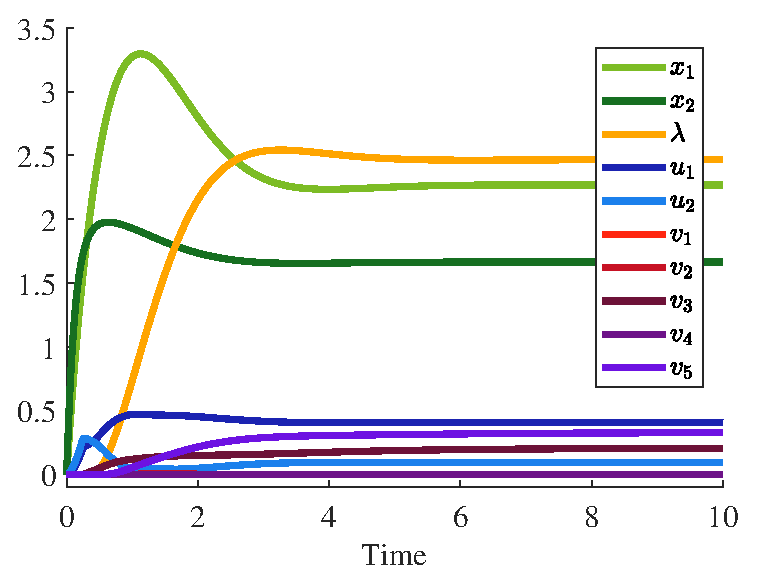
\includegraphics[scale=0.55]{trajectories_intersection.eps}
\vspace{-1.5mm}
\caption{\rev{Trajectories of $\mathcal{RO}$ dynamics for robust QP problem with intersection of ellipsoids uncertainty set in Example A.}}
\label{trajectories_norm_intersection}
\end{center}
\end{figure}
\begin{figure}
\begin{center}
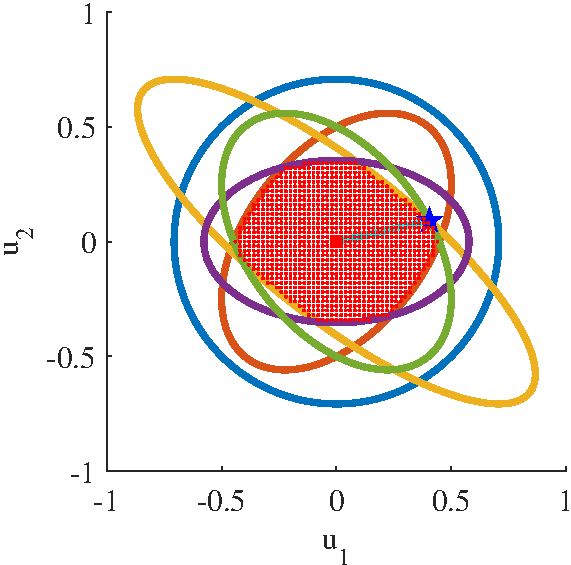
\includegraphics[scale=0.55]{ellipsoids}
\vspace{-1.5mm}
\caption{\rev{Uncertainty set for Example A plotted in $u_
2$-$u_1$ space. Big red point at the origin represents the initial point of $u$ in $\mathcal{RO}$ dynamics and blue star depicts the optimal value of $u$ on the intersection of two ellipsoids derived by our method. Small red grid points are the $1115$ sampled points from the uncertainty set in randomized scenario method \cite{calafiore2004} to compare with our method.}}
\vspace{-8mm}
\label{ellipsoids}
\end{center}
\end{figure}

\subsection{Robust Nonlinear Optimization with no RC}\label{norc.sec}

Consider the following robust nonlinear optimization problem
\begin{align} \label{ro_simulation_3}
&\min_{x \in \mathbf{R}^2} \;f(x):=\frac{1}{2}(x_1-1)^2+\frac{1}{2}(x_2-2)^2\\
&\;\;\;\text{s.t.}\;\;\max_{u\in {\cal U}} u^\top \left[\begin{array}{ccl}e^{x_1^2}\\e^{x_2^2} \end{array}\right] \leq b\;,\;\nonumber
\end{align}
where $x \in \mathbf{R}^2$, and $u=[u_1, u_2]^\top \in \mathbf{R}^2$, for which, the strictly convex uncertainty set is described by
\begin{align} \label{uncertasinty_example3}
{\cal U}:=\{u \in \mathbb{R}^{2}:e^{u_j^2}+u_j e^{\frac{1}{u_j}} \leq \rho_j\;,\; j=1,2\}\;.
\end{align}
As stated in \cite{bental20152} and \cite{gorissen20152}, there is no closed-form convex conjugate for the constraint (convex in $x$) in (\ref{ro_simulation_3}) and no closed-form conjugate for the convex uncertainty set in (\ref{uncertasinty_example3}). This is the third case in \cite[~Table 1]{gorissen20152}, for which there is no known method for obtaining RC. However, by writing the Lagrangian function as
\begin{align*}
\mathcal{L}=&\frac{1}{2}(x_1-1)^2+\frac{1}{2}(x_2-2)^2\\
&+\lambda \Big(u^\top \Big[\begin{array}{ccl}e^{x_1^2}\\e^{x_2^2} \end{array}\Big]-b-v^\top \Big[\begin{array}{cc} e^{u_1^2}+u_1 e^{\frac{1}{u_1}}-\rho_1 \\ e^{u_2^2}+u_2 e^{\frac{1}{u_2}}-\rho_2 \end{array}\Big]\Big)\;,
\end{align*}
where $h_j(u_j)=e^{u_j^2}+u_j e^{\frac{1}{u_j}}-\rho_j$ for $j=1,2$ as defined in the previous example, we can form the $\mathcal{RO}$ dynamics for the RNO problem (\ref{ro_simulation_3}) as
\begin{align*}
&\dot x=-\Big[\begin{array}{ccl} x_1-1 \\ x_2-2 \end{array}\Big]-\hat{\lambda}\; \Big[\begin{array}{cc} 2 x_1 e^{x_1^2} & 0 \\ 0 & 2 x_2 e^{x_2^2}\end{array}\Big]u \nonumber\;,\\
&\dot {\hat{\lambda}} = \Big[u^\top \Big[\begin{array}{cc} e^{x_1^2}\\ e^{x_2^2}\end{array}\Big]-b- \sum_{j=1}^2 \big(v_j(e^{u_j^2}+u_j e^{\frac{1}{u_j}}-\rho_j)\big)\Big]_{\hat{\lambda}}^{\varepsilon+}\nonumber\;,\\
&\dot u=\Big[\begin{array}{cc} e^{x_1^2}\\ e^{x_2^2}\end{array}\Big]- \sum_{j=1}^2(2u_j e^{u_j^2}+e^{\frac{1}{u_j}}-\frac{1}{u_j} e^{\frac{1}{u_j}}) v_j\nonumber\;,\\
&\dot v=\Big[\hat{\lambda}\; \Big[\begin{array}{cc} e^{u_1^2}+u_1 e^{\frac{1}{u_1}}-\rho_1 \\ e^{u_2^2}+u_2 e^{\frac{1}{u_2}}-\rho_2 \end{array}\Big] \Big]_{v}^+\nonumber\;,
\end{align*}
according to $\mathcal{RO}$ dynamics (\ref{pd_dynamics_0}) where $\hat{\lambda}=\lambda+\varepsilon$. Similarly to the previous example, we can set $\varepsilon$ to zero according to Remark \ref{active_inactive_constraint_rem} as the constraint is active. Fig. \ref{trajectories_nonlinear_exp_no_RC} shows the trajectory plot for $\rho_1=10$, $\rho_2=20$, and all the states initialized at $1$. The robust optimal solution is $[0.5271, 0.7916]$ and the optimal cost value is $0.8419$. We observe that the optimal value for $u$, which is $[1.4020, 1.6824]$ lies on the boundary of the uncertainty set. For positive values of $\varepsilon$, the trajectory and convergence value of $\lambda$ may change, but the solution $x$ remains the same as the constraint is active.

\rev{For this problem with highly nonlinear uncertainty constraints $e^{u_j^2}+u_j e^{1/u_j} \leq \rho_j$, no closed-form robust counterpart exists \cite{bental2009,gorissen20152}, making RC-based methods inapplicable. We compared our approach with scenario-based sampling \cite{calafiore2004}: using CVX, 168 scenarios yielded solution $[0.5376, 0.8193]$ with cost $0.8039$ (2.3s), 500 scenarios gave $[0.5312, 0.8024]$ with cost $0.8287$ (8.7s), and 1000 scenarios produced $[0.5289, 0.7953]$ with cost $0.8371$ (31.2s). Our method obtained the exact solution $[0.5271, 0.7916]$ with optimal cost $0.8419$ in 0.8s integration time—40× faster than the 1000-scenario approximation while providing the exact solution rather than an approximation.}

\rev{This example illustrates a key advantage of our approach: the dynamics naturally handle nonlinear uncertainty constraints through gradient terms $\nabla_{u_j} h_j(u_j)$, achieving exact convergence where other methods either fail completely (when RC cannot be derived) or require computationally expensive approximations with complexity $O(N^3n^3)$ for $N$ scenarios versus our $O(n^2)$ scaling.}
\begin{figure}
\begin{center}
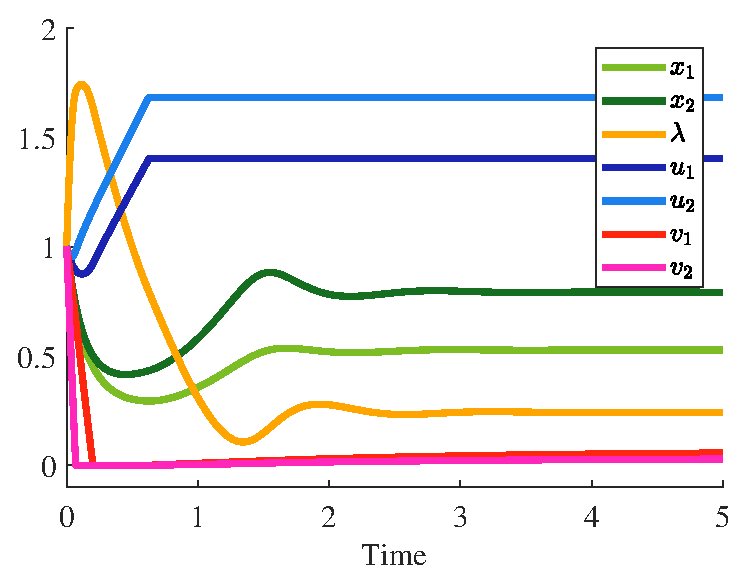
\includegraphics[scale=0.55]{trajectories_nonlinear_exp_no_RC.eps}
\caption{\rev{Trajectory of $\mathcal{RO}$ dynamics for robust nonlinear optimization problem (\ref{ro_simulation_3}) in Example B.}}
\label{trajectories_nonlinear_exp_no_RC}
\end{center}
\end{figure}

\subsection{Robust Dynamic Location Problem}
We now consider the optimal cooperative and robust self-placement of autonomous vehicles, modeled as first-order kinematic points, to monitor multiple targets (initially assumed static). This is a dynamic generalization of a classical facility location problem \cite{farahani2009} and here we provide a solution to the robust formulation of this problem using $\mathcal{RO}$ dynamics. The optimization problem is described by an undirected graph with $N$ nodes and a set of edges ${\mathbb E}$. Among these nodes, the first $N_1$ nodes represent the fixed positions of the targets (also referred to as anchors), while the remaining $N_2 = N - N_1$ nodes represent the mobile agents. Each node $x_i\in \mathbb{R}^2$ denotes the location of an anchor or an agent. The anchors $x_1,\cdots,x_{N_1}$ have fixed positions and the agents $x_{N_1+1},\cdots,x_{N}$ are mobile and can adjust their positions. The problem is to find the locations of the sensor nodes $x_{N_1+1},\cdots, x_N$ to minimize the following cost
\begin{align*}
g(x_1,..,x_{N_1})=\min_{x_{N_1+1},\cdots,x_N} \sum_{(i,j)\in {\mathbb E}}
f_{ij}(x_i, x_j)\;,
\end{align*}
which is the sum of some measure of ``length'' for each link. This problem and its generalizations have many applications \cite{boyd2004}, and can be solved efficiently and in a distributed fashion in continuous time \cite{wang2011}. Leaving the sensor nodes (agents) mobile and capable of computation in distributed mode, we obtain a distributed dynamical version \emph{real-time} of the optimal placement. The sensor nodes, through local interactions, cooperate to find and move toward their globally optimal locations autonomously.

The problem can also be under a set of constraints for the position of agents $x_{N_1+1},\cdots,x_{N_1}$ to be in a specified convex set. Specifically, we consider the following robust location and placement problem
\begin{align*}
    &\min_{x_{N_1+1},\cdots,x_N} \sum_{(i,j)\in {\mathbb E}} \frac{1}{2}\; w_{ij} \parallel x_i - x_j \parallel_2^2\\
    &\;\;\text{s.t.}\;\;\underset{u_i\in \mathcal{U}_i}{\max} (a_i+P_i u_i)^\top x_i \leq b_i, \; i={N_1+1},\cdots,N\;,
\end{align*}
where the uncertainty $u_i$ lies in $\mathcal{U}_i = \parallel u_i \parallel_2^2\; \leq \rho_i^2$ and $x_{N_1}+1,\cdots,x_{N}$ are moving agents. The $\mathcal{RO}$ dynamics for this problem can be derived as follows for $i=N_1+1,\cdots,N$
\begin{align*}
\left\{
\begin{array}{cl}
\vspace{2mm}
&\dot{x}_i=\sum_j w_{ij} (x_i-x_j)-\hat \lambda_i \; (a_i+P_i u_i)\\
\vspace{2mm}
&\dot{\hat \lambda}_i=[(a_i+u_i P_i)^\top x_i-P_i u_i^\top c_i-b_i-v_i\; \mathcal{U}_i]_{\hat \lambda_i}^{\varepsilon+}\\
\vspace{2mm}
&\dot{u}_i=P_i^\top (x_i-c_i)-2v_i u_i\\
\vspace{2mm}
&\dot{v}_i=[\hat \lambda_i\; \mathcal{U}_i]
\vspace{2mm}
\end{array}\right..
\end{align*}
Note that this problem is naturally distributed and our dynamics reflects the distributed structure. We consider the setup shown in the figure below with five anchors and four agents. The figure also shows the (fixed) interconnection graph among all the elements of the problem. In this academic example, we consider the presence of a linear constraint defining the half-space where the agents can be. The constraint is simply
\begin{align*}
{\bf 1}'x_i\leq 2.5, \;\; i=N_1+1,\cdots,N\;,
\end{align*}
for all the agents.
In addition, we would like the agents to find robust locations based on the uncertainty on the nominal slope $45^o$ of the nominal constraint. Namely
\begin{align*}
{\bf 1}'x_i+u_iP'x_i\leq 2.5,\;\; i=N_1+1,\cdots,N\;,
\end{align*}
where $P'=\begin{bmatrix}1&-1\end{bmatrix}$ and $\|u_i\|_2^2\leq \rho^2$. For example, when $\rho=1$, the constraint can be any line passing through $x'=(1.25,\,1.25)$, including the horizontal and vertical ones. The figure also shows the nominal linear constraint. The location of the shown agents is the optimal robust one w.r.t. the constraint being perturbed by the uncertainty $u_i$ with $\|u_i\|_2^2\leq 0.1$.


First, agents start at their initial locations at the origin (white circle), and their paths converge to the optimal robust location for $\rho^2=0.1$. Such locations are indicated by full-colored circles. We see that agents $1$ and $4$ (blue and green) are on the boundary of the robust feasible set identifiable with the larger sector in the figure. The uncertain constraint is not active for the other agents. However, their optimal location is indirectly influenced by the robust constraint active in agents $1$ and $4$ as all agents and anchors are interconnected.

In the next phase of the simulation, we rotate the location of the anchors clockwise at constant speed. Although agents only react to their local neighbors (agents/anchors), the interconnected dynamical system shows the ability to globally track the coordinated motion of the anchors within the robust feasible set. It is interesting to notice that the boundary of the feasible set is not defined a priori or hard-coded in the simulation, but it emerges from the interactions built in the dynamical system. Finally, after some time, the uncertainty changes and increases with size $\rho^2=1$ at time $t=300$. This implies that no location should be feasible above the horizontal line passing through $(1.25,1.25)$ and on the right of the vertical line passing through the same point. The location of the agents when the uncertainty changes is indicated by black empty circles. We note that, when the uncertainty changes, the nodes $1$, $2$, and $3$ are located outside the new robust feasible set and, with a transient correction, move inside the robust SW quadrant for the rest of the time.

This example showcases the ability of the dynamical system to track changes online and adapt to uncertainty changes over time. We have obtained the behavior shown by appropriate scaling of the various differential equations involved. Note that the convergence is not affected by positive scaling of the differential equations. A relatively larger scaling on the dual variables in charge of the constraints makes the system response more reactive toward feasibility and more sensitive toward uncertainty changes. We leave to future research the systematic design of the optimization system for the desired real-time behavior.

\begin{figure}
\begin{center}
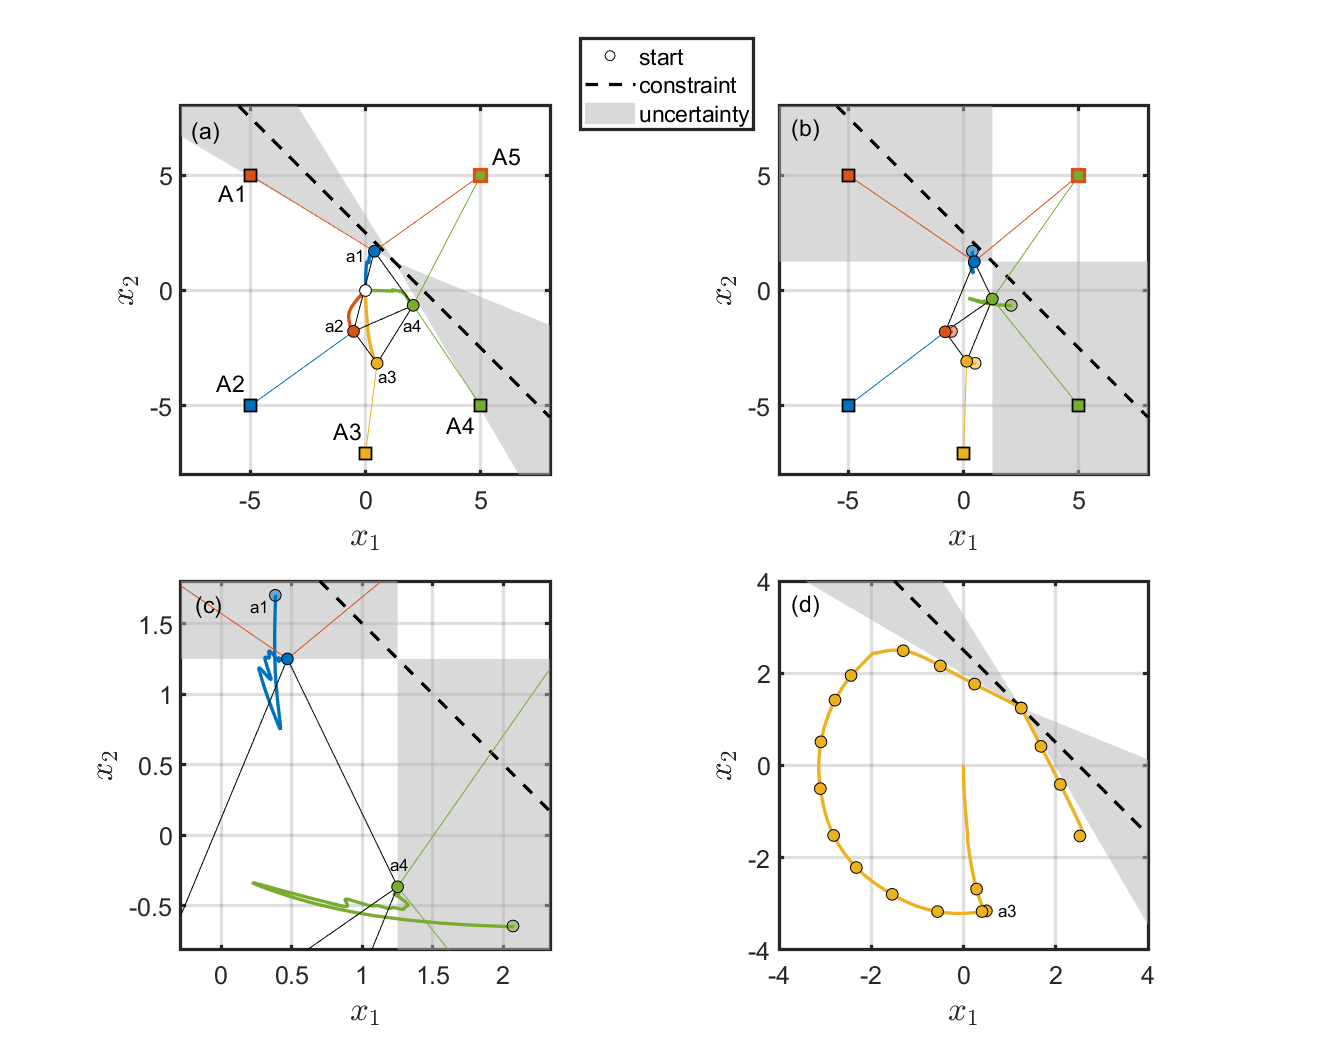
\includegraphics[scale=0.26]{simulation_figure_finalv3.png}
\vspace{-1.5mm}
\caption{\rev{Locations of agents and anchors, interactions between agents and anchors, and nominal linear constraint in Example C.}}
\label{fig_points}
\end{center}
\end{figure}

\section{Conclusions}\label{section_conclusions}


\rev{This paper introduced $\mathcal{RO}$ dynamics for solving robust optimization problems through continuous-time evolution. The method achieves significant efficiency and generalization improvements while providing exact solutions for problems where robust counterparts are intractable. Applications to machine learning robustness, adversarial training, and large-scale distributed optimization represent promising future directions. Open challenges include convergence rate characterization and extension to non-convex settings.}
\section{Appendix} \label{section_appendix}

\subsection{Lemma \ref{saddle.lem} [Saddle property]}
Essentially, we want to show that
\begin{align*}
\mathcal{L}(x^\star,\lambda,u,v^\star)\leq \mu \leq \mathcal{L}(x,\lambda^\star,u^\star,v)\;.
\end{align*}
Under Assumption \ref{assume_feasible}, an optimal solution $x^\star$ exists and based on Assumption \ref{assume1}, this optimal solution is unique as $f_0(x,u_0)$ is strictly convex in $x$ for any $u_0 \in\mathcal{U}_0$. Consider any optimal solution $(x^\star,\lambda^\star,u^\star,v^\star)$ for $\mathcal{RO}$ problem (\ref{dual.eq}).

\noindent
For each of the lower level optimizations, let
\begin{align*}
\eta_i=\max_{u_i\in \mathcal{U}_i}f_i(x^\star,u_i)=f_i(x^\star,u_i^\star)=
\tilde\mathcal{L}_i(x^\star,u_i^\star,v_i^\star),\; i\in[N]\;.
\end{align*}
From the corresponding saddle property, it follows that for all $u_i$, $i\in[N]$,
\begin{equation}\label{xxlb.eq}
f_i(x^\star,u_i)-(v_i^\star)^\top h_i(u_i)\leq \eta_i\;.
\end{equation}
From the upper level saddle property, for all $\lambda_i\geq 0$, $i\in[N]^+$,
\begin{align*}
\eta_0+\sum_i(c_i+\lambda_i)\eta_i\leq f_0(x^\star,u_0^\star)+\sum_{i=1}^N(c_i+\lambda_i^\star)\eta_i=\mu\;.
\end{align*}
Substituting the lower bound on $\eta_i$, (\ref{xxlb.eq}), in the left hand side, it follows that for all $u_i, i\in[N]$ and $\lambda_i\geq 0, i\in[N]^+$,
\begin{align*}
&\mathcal{L}(x^\star,\lambda,u,v^\star)\\
= &f_0(x^\star,u_0)-(v_0^\star)^\top h_0(u_0)\\
& +\sum_{i=1}^
N(c_i+\lambda_i)(f_i(x^\star,u_i)-(v_i^\star)^\top h_i(u_i))\\
\leq &\;\mu\;,
\end{align*}
where we have used $c_i+\lambda_i\geq 0$. We next use lower saddle property in the other direction, namely, for all $v_i\geq 0$,
\begin{align*}
\eta_i=f_i(x^\star,u_i^\star)=f_i(x^\star,u_i^\star)-(v_i^\star)^\top h_i(u_i^\star)\\
\leq f_i(x^\star,u_i^\star)-(v_i)^\top h_i(u_i^\star)\;,
\end{align*}
which implies that for all $v_i\geq 0$, $-v_i^\top h(u^\star)\geq 0$, $i\in[N]$.\\
Using this property and the fact that $(c_i+\lambda_i^\star)\geq 0$, it follows that for all $v_i\geq 0$, $i^+_{[N]}$,
\begin{equation}\label{xxub.eq}
-(v_0)^\top h_0(u_0^\star)-\sum_{i=1}^N(c_i+\lambda_i^\star)(v_i)^\top h_i(u_i^\star)\geq 0\;.
\end{equation}

\noindent
The upper level saddle property implies
\begin{align*}
\mu\leq f_0(x,u_0^\star)+\sum_{i=1}^N(c_i+\lambda_i^\star)f_i(x,u_i^\star)
\end{align*}
for all $x$. Combining this with (\ref{xxub.eq}), we obtain
\begin{align*}
\mu&\leq f_0(x,u_0^\star)-(v_0)^\top h_0(u_0^\star)\\
&+\sum_{i=1}^N(c_i+\lambda_i^\star)(f_i(x,u_i^\star)-(v)^\top h_i(u_i^\star))\\
&=\mathcal{L}(x,\lambda^\star,u^\star,v)
\end{align*}
for all $x$ and $v_i\geq 0, i\in[N]$.

\subsection{$\mathcal{RO}$ dynamics solutions properties}\label{existence.sec}
$\mathcal{RO}$ dynamics (\ref{pd_dynamics}) can be viewed as switched dynamical system with a discontinuous right-hand side. The conditions guaranteeing the existence and uniqueness of the solution and continuity w.r.t. initial conditions, for a general discontinuous dynamical system are provided in \cite[Theorem~2.5]{nagurney2012projected}. In this section, we show that our $\mathcal{RO}$ dynamics (\ref{pd_dynamics}) satisfies the refined conditions presented in \cite{cherukuri2016}.

To prove the existence and uniqueness of solutions for (\ref{pd_dynamics}), and also the continuity of solutions w.r.t. the initial conditions, there are two main steps. The first step is showing that $\mathcal{RO}$ dynamics is a particular case of projected dynamical systems. The second step requires $\mathcal{RO}$ dynamics (\ref{pd_dynamics}) satisfying the monotonicity property, which is our main result.

\begin{definition} \label{projection_operator} (Projection operator)
If ${\cal K}$ is a closed convex set, for any point $\bar y \in \mathbb R^q$, the point projection of $\bar y$ on the set ${\cal K}$ can be written as
\begin{align*}
\text{proj}_{\cal K}(\bar y)=\text{argmin}_{y \in {\cal K}} \parallel y-\bar y \parallel\;.
\end{align*}
For $\bar y \in \mathbb R^n$ and $y \in {\cal K}$, vector projection of $\bar y$ at $y$ w.r.t. ${\cal K}$ is
\begin{align}
\label{projection_operator}
\Pi_{\cal K}(y,\bar y) = \text{lim}_{\delta \rightarrow 0^+} \frac{\text{proj}_{\cal K}(y+\delta \bar y)-y}{\delta}\;.
\end{align}
\end{definition}

Note that the map $\text{proj}_{\cal K}$ is Lipschitz on $\mathbb R^q$ with constant $L=1$ \cite[Proposition~2.4.1]{clarke1983}.

\begin{definition} \label{projected_dynamical_system} [Projected dynamical system \cite{nagurney1996}]
Considering a differential equation $\dot y=F(y)$ with $F:\mathbb R^q \rightarrow \mathbb R^q$, the associated projected dynamical system is defined as
\begin{align}
\label{projected_dynamics}
\dot y = \Pi_{\cal K}(y,F(y)),\; y(0) \in {\cal K}\;.
\end{align}
\end{definition}

\begin{lemma} \label{projected} ($\mathcal{RO}$ dynamics as a projected dynamics)
$\mathcal{RO}$ dynamics (\ref{pd_dynamics}) can be written as a projected dynamical system according to Definition \ref{projected_dynamical_system}.
\end{lemma}
\begin{proof}
The proof of Lemma \ref{projected} follows along the lines of the construction outlined in \cite{cherukuri2016}. Details omitted.
\end{proof}

\begin{remark}[\rev{Projected Dynamics Foundation}]
\rev{The following proposition ensures: (i) existence despite discontinuities from projections, (ii) uniqueness via Lipschitz property, (iii) continuous dependence on initial conditions, (iv) validity of Lyapunov analysis for Theorem \ref{maintheorem}.}
\end{remark}

\begin{proposition} \label{proposition_projected}
If $F$ in the projected dynamical system (\ref{projected_dynamics}) is Lipschitz on ${\cal K}$, we have the following existence, uniqueness, and continuity w.r.t. the initial condition results for the solutions of the projected dynamics (\ref{projected_dynamics}):
\begin{enumerate}
\item For any $y_{0} \in {\cal K}$, there exists a unique solution $t \rightarrow y(t)$ of the projected system (\ref{projected_dynamics}) with $y(0)=y_{0}$ in $[0,\infty)$.
\item Consider a sequence of points $\{y_{k}\}_{k=1}^\infty \subset {\mathcal K}$ with $\lim_{k \rightarrow \infty} y_k=y$. Then, the sequence of solutions $\{t \rightarrow \gamma_k(t)\}_{k=1}^\infty$ of the projected dynamics (\ref{projected_dynamics}) with $\gamma_k(0)=y_k$ for all $k$, converges to the solution $t \rightarrow \gamma(t)$ of (\ref{projected_dynamics}) with $\gamma(0)=y$ uniformly on every compact set of $[0,\infty)$.
\end{enumerate}
\end{proposition}
The ability to write $\mathcal{RO}$ dynamics (\ref{pd_dynamics}) as a projected dynamical system along with the monotonicity property is used in the proof of the existence, uniqueness and continuity of the solutions of the set ${\mathbb S}$.

\begin{lemma} \label{uniq_exis}
(Existence, uniqueness and continuity of solutions)
$\gamma:[0,T) \rightarrow {\mathbb S}$ is defined as a Caratheodory solution of $\mathcal{Z}^{\mathcal{RO}}$ in the interval $[0,T)$ if $\gamma$ is absolutely continuous on $[0,T)$ and satisfies $\dot \gamma(t)=\mathcal{Z}^{\mathcal{RO}} (\gamma(t))$ almost everywhere in $[0,T)$.
Under Assumptions \ref{assume1} and \ref{assume_feasible}, and starting from any point $z\in \mathbb S$, a unique solution to $\mathcal{RO}$ dynamics (\ref{pd_dynamics}) exists and remains in $\mathbb S \cap V^{-1}(\leq V(z))$. Also, if a sequence of points $\{z_k\}_{k=1}^\infty \subset {\mathbb S}$ converges to $z$ as $k \rightarrow \infty$, the sequence of solutions $\{t \rightarrow \gamma_k(t)\}_{k=1}^\infty$ of $\mathcal{Z}^{\mathcal{RO}}$ starting at these points (that is, $\gamma_k(0)=z_k$ for all $k$) converge uniformly to the solution $t \rightarrow \gamma(t)$ on every compact set of $[0,\infty)$.
\end{lemma}
The proof of this lemma follows closely along the lines of proof for the existence and uniqueness of solution for the primal-dual dynamical system from \cite[Lemma~4.3]{cherukuri2016}.


\subsection{Theorem \ref{RO_ROperturbed}}

Based on the optimal solution $x^\star$ for $\mathcal{RO}$ problem,
\begin{align*}
\mu=\min_{\mathcal{F}_i(x)\leq  0} \mathcal{F}_0(x)\;,\; \mu=\mathcal{F}_0(x^\star)\;.
\end{align*}
As the cost function of $\mu_\varepsilon$ is smaller than or equal to that of $\mathcal{RO}$ and the feasible sets of the two problems are equal,
\begin{equation}\label{ub.eq}
 \mu_\varepsilon-\mu\leq 0\;.
\end{equation}
Since $x^\star$ minimizes $\mathcal{F}_0(x)$ over the constraint set, $\mu=\mathcal{F}_0(x^\star)\leq \mathcal{F}_0(x_\varepsilon^\star)$.
Adding and subtracting $\varepsilon\sum_{i=1}^n\mathcal{F}_i(x^\star_\varepsilon)$
in the right-hand side (RHS) and using (\ref{ub.eq}) yields $\varepsilon \sum_{i=1}^N{\cal F}_{i}(x_\varepsilon^\star)\leq
\mu_\varepsilon-\mu\leq 0$\;.

Following a similar argument as before by comparing $\mu(\varepsilon_0)$ and $\mu_\varepsilon$ for $\varepsilon_0\geq \varepsilon$, we now let
\begin{align*}
&\mu_\varepsilon=\tilde{{\cal F}}_0(x^\star_\varepsilon)=\mathcal{F}_0(x^\star_\varepsilon)+\varepsilon\sum_{i=1}^N\mathcal{F}_i(x^\star_\varepsilon)\;,\\
&\mu(\varepsilon_0)=\tilde{{\cal F}}_0(x^\star_{\varepsilon_0})+\delta\sum_{i=1}^N\mathcal{F}_i(x^\star_{\varepsilon_0})\;,
\end{align*}
where $\delta=\varepsilon_0-\varepsilon$. Then, $\mu_\varepsilon\geq \mu(\varepsilon_0)$\;,
but because $x_\varepsilon^\star$ is optimal for $\mu_\varepsilon$\;, we have
$\tilde{{\cal F}}_0(x^\star_\varepsilon)\leq \tilde{{\cal F}}_0(x^\star_{\varepsilon_0})$.
As $x^\star_\varepsilon$ is feasible for $\mu(\varepsilon_0)$, \begin{align*}
\tilde{{\cal F}}_0(x^\star_{\varepsilon_0})+\delta\sum_{i=1}^N\mathcal{F}_i(x^\star_{\varepsilon_0})=\mu(\varepsilon_0)\leq \tilde{{\cal F}}_0(x^\star_{\varepsilon})+\delta\sum_{i=1}^N\mathcal{F}_i(x^\star_{\varepsilon})\;.
\end{align*}
Combining the two inequalities,
\begin{align*}
\delta\sum_{i=1}^N\mathcal{F}_i(x^\star_{\varepsilon_0})-\delta\sum_{i=1}^N\mathcal{F}_i(x^\star_{\varepsilon})\leq \tilde{{\cal F}}_0(x^\star_{\varepsilon})-\tilde{{\cal F}}_0(x^\star_{\varepsilon_0})\leq 0\;,
\end{align*}
which implies that $\sum_{i=1}^N\mathcal{F}_i(x^\star_{\varepsilon_0})\leq \sum_{i=1}^N\mathcal{F}_i(x^\star_{\varepsilon})$. Thus,
\begin{equation}\label{limi.eq}
\varepsilon\sum_{i=1}^N{\cal F}_{i}(x_{\varepsilon_0}^\star)\leq
\varepsilon\sum_{i=1}^N{\cal F}_{i}(x_{\varepsilon}^\star)\leq
\mu_\varepsilon-\mu \leq 0\;.
\end{equation}
Since $\sum_{i=1}^N{\cal F}_{i}(x_{\varepsilon_0}^\star)=\frac{\mu(\varepsilon_0)-\mathcal{F}_0(x^\star_{\varepsilon_0})}{\varepsilon_0}$ is bounded, we have
\begin{equation}\label{limi2.eq}
\varepsilon\sum_{i=1}^N{\cal F}_{i}(x_{\varepsilon_0}^\star)\leq
\mu_\varepsilon-\mu\leq 0\;,
\end{equation}
which means that $\mu_\varepsilon$ converges to $\mu$ as $\varepsilon\to 0$.

To prove the second part of the theorem, that is, $x^\star_\varepsilon \to x^\star$ as $\varepsilon \to 0$, consider any sequence $\{\varepsilon_n\}$ converging to $0$. Let $\{x^\star_{n}\}$ be the corresponding sequence of optimal solutions for $\mu(\varepsilon_n)$.

As ${\cal C}$ is compact and the same for both perturbed and original problem, $x^\star_{n}\in {\cal C}$ is bounded.  Therefore, there exists a convergent sub-sequence $x_{n_t}^\star$ that converges to, say, $\hat{x}\in {\cal C}$, as $\varepsilon_{n_t} \to 0$, since ${\cal C}$ is closed by assumption.

This implies that
$\mathcal{F}_0(x_{n_t}^\star) \to \mathcal{F}_0(\hat{x})\;,$ since $\mathcal{F}_0(x)$ is continuous.
Because $\hat{x}$ is feasible, $\mathcal{F}_0(\hat{x})\geq \mu$.
However,  $\mathcal{F}_0(\hat{x})>\mu$ is impossible since
$
\mu(\varepsilon_{n_t})\to \mu
$,
from the first part of the proof, and $\displaystyle\mu(\varepsilon_{n_t})=\mathcal{F}_0(x^\star_{n_t})+\varepsilon_{n_t}\sum_{i=1}^N{\cal F}_{i}(x_{n_t}^\star)\to \mathcal{F}_0(\hat{x})$, since from (\ref{limi.eq}) and (\ref{limi2.eq}), $\displaystyle\lim_{\varepsilon_{n_t}\to 0}
\varepsilon_{n_t}\sum_{i=1}^N{\cal F}_{i}(x_{\varepsilon_{n_t}})=0$\;.

Therefore, $\mathcal{F}_0(\hat{x})=\mu=\mathcal{F}_0(x^\star)$. Since $f(x)$ is strictly convex, $\hat{x}=x^\star$. Since every convergent sub-sequence converges to $x^\star$, the whole sequence converges to it. Since the sequence was arbitrary, we have that $x^\star_\varepsilon\to x^\star$ as $\varepsilon\to 0$\;.


\bibliography{2.References}
\bibliographystyle{ieeetr}
\begin{IEEEbiography}
[{
\includegraphics[width=1in,height=1.25in,clip,keepaspectratio]{k1.jpg}}]
{Keivan Ebrahimi} received bachelor's and master's degree in electrical engineering from Sharif University of Technology, Tehran, Iran in 2012 and 2014. He is a Ph.D. candidate in electrical and computer engineering at Iowa State University (ISU), Ames, IA, USA. He is currently a principal data scientist at Tarana Wireless in Milpitas, CA, USA. He received the College of Engineering fellowship at Iowa State University in 2015 and has been selected for the Rock Star Spot Award for stellar contribution and performance in View Inc. COVID-SENSE product, May 2020. He filed three patents to the United States Patents and Trademarks Office for “Environmental Adjustment using Artificial Intelligence”, “Identifying and Reducing Health Risks and Tracking Occupancy in a Facility”, and “Immersive Collaboration of Remote Participants via Media Displays”. His research interests include adversarial machine learning and deep learning, computer vision, robust optimization, control theory and dynamical systems.
\end{IEEEbiography}

\begin{IEEEbiography}
[{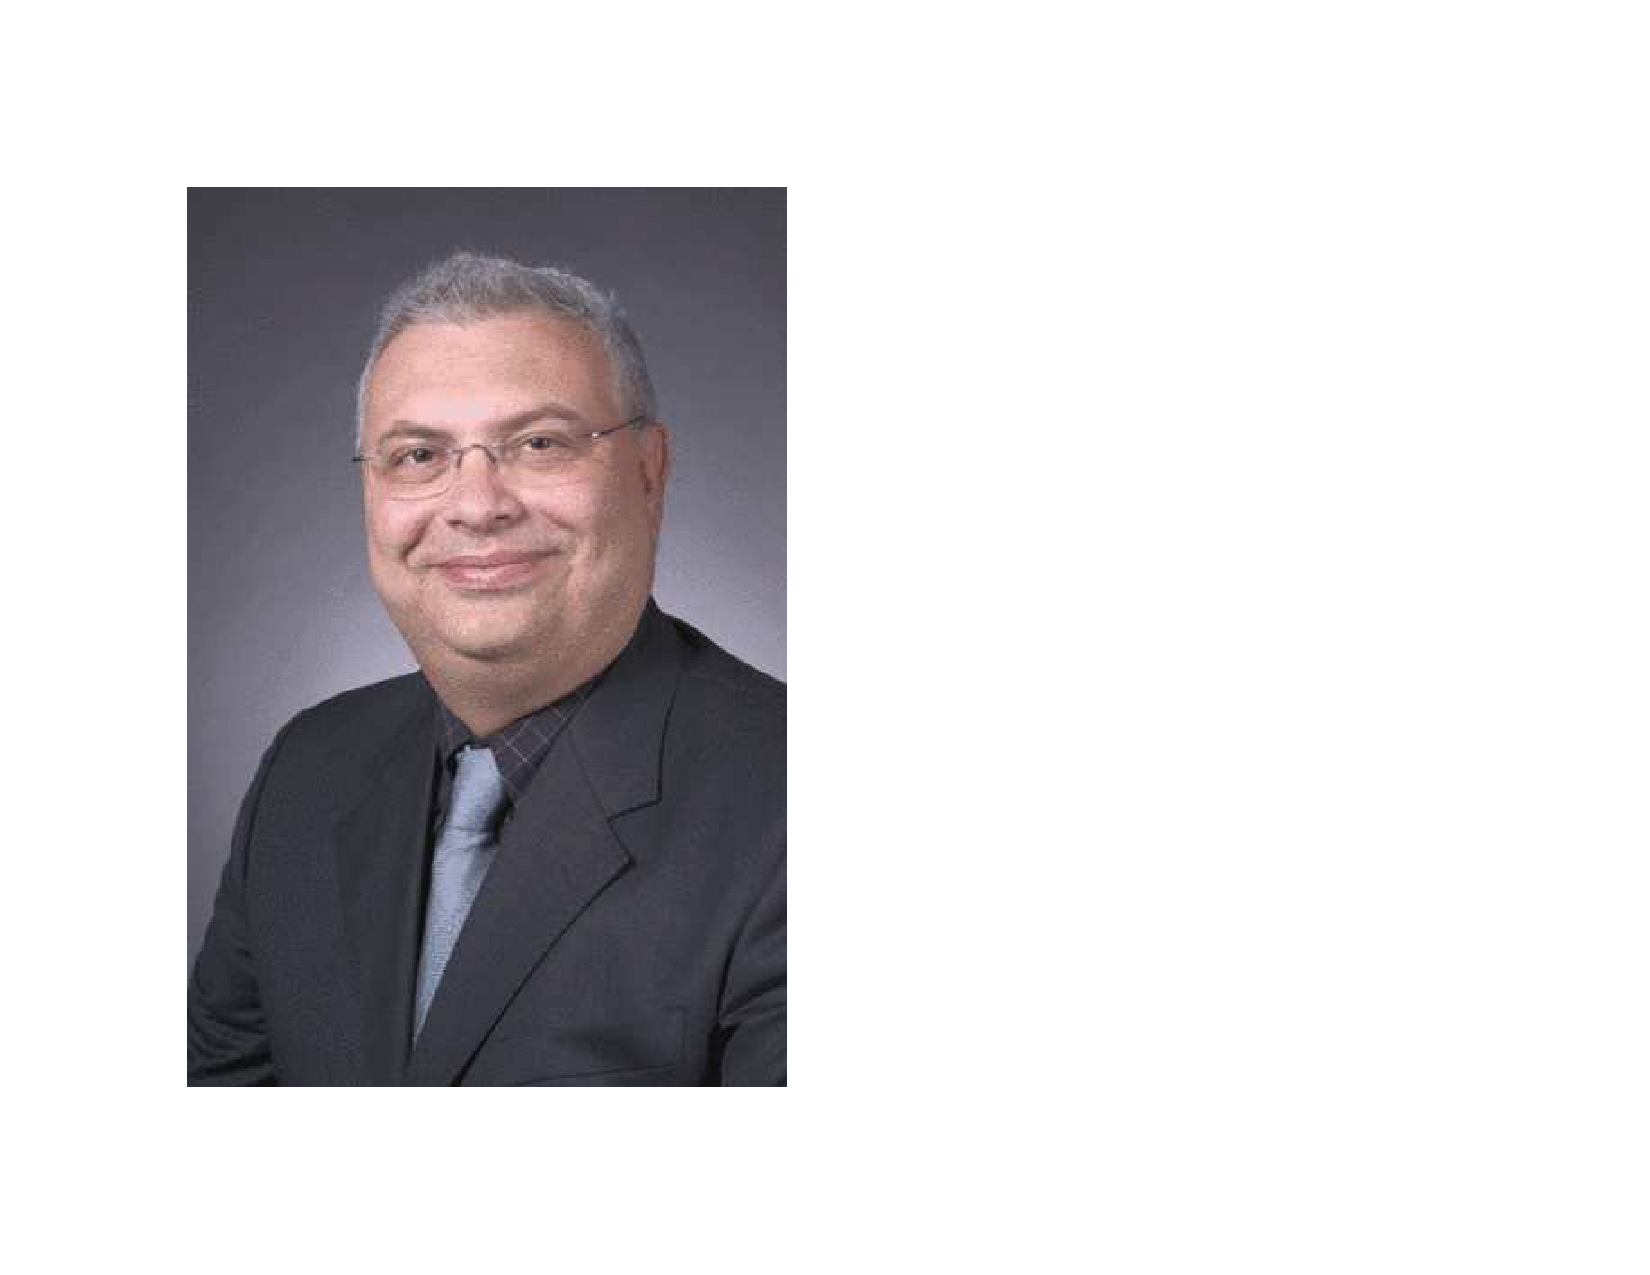
\includegraphics[width=1in,height=1.25in,clip,keepaspectratio]{elia.pdf}}]
{Prof. Nicola Elia} received the Laurea degree in Electrical Engineering from the Politecnico di Torino, Turin, Italy in 1987 and the Ph.D. degree in Electrical Engineering and Computer Science from the Massachusetts Institute of Technology (MIT), Cambridge, MA, USA in 1996. He is currently the Vincentine-Hermes-Luh Chair Professor of Electrical and Computer Engineering at the University of Minnesota (UMN), Twin Cities, MN, USA. Before joining UMN in 2018, and since 1999, he was a faculty with the department of Electrical and Computer Engineering at Iowa State University, Ames, IA, USA. He was a Postdoctoral Associate at the Laboratory for Information and Decision Systems at MIT from 1996 to 1999. He was a Control Engineer with the Fiat research Center, Turin, Italy, from 1987 to 1990. Dr. Elia received the NSF Career Award and he is a Fellow of the IEEE. His research interests include computational methods for controller design, communication systems with access to feedback, control with communication constraints, and network distributed systems.
\end{IEEEbiography}

\begin{IEEEbiography}
[{
\includegraphics[width=1in,height=1.25in,clip,keepaspectratio]{umesh.jpeg}}]
{Prof. Umesh Vaidya} received the Ph.D. degree in mechanical engineering from the University of California at Santa Barbara, Santa Barbara, CA, in
2004. He was a Research Engineer at the United Technologies Research Center (UTRC), East Hartford, CT, USA. He is currently a professor in the Department of Mechanical Engineering, Clemson University, S.C., USA. Before joining Clemson University in 2019, and since 2006, he was a faculty with the department of Electrical and Computer Engineering at Iowa State University. He is the recipient of 2012 National Science Foundation CAREER award. His current research interests include dynamical systems and control theory.
\end{IEEEbiography}

% Switch to single column for reviewer comments and responses
\onecolumn

\section*{Reviewer Comments}

\subsection*{Reviewer 4}

This manuscript proposes a dynamical system-based approach for solving robust optimization problems in a general convex-concave framework. This proposed approach offers a novel solution to robust optimization problems by introducing a continuous-time dynamical system. Additionally, the proposed dynamical system-based approach offers better properties compared to traditional approaches and demonstrates the potential to solve a broad range of robust optimization problems in a decentralized manner. Some detailed comments are given as follows.

\textcolor{reviewerred}{\textit{The improvements compared to the existing results are also unclear, which makes it difficult to evaluate the contribution of this article.}}

\textcolor{reviewerred}{\textit{There are some language and grammar issues in this paper and the authors need to revise their paper properly.}}

The definite article in the captions of all figures is suggested to be omitted. In general, the definite article in the title should be omitted.

The italics of many formulas in this manuscript are not standard, and there are some inconsistent phenomena.

There are issues with the quotation marks in the manuscript.

\subsection*{Reviewer 5}

This paper proposes a novel continuous-time dynamical system, termed RO dynamics, for solving robust optimization (RO) problems in a convex-concave framework. While the approach is innovative and has potential, the manuscript requires significant revisions to improve clarity, technical rigor, and presentation. Below are specific comments and suggestions for improvement.

\textcolor{reviewerred}{\textit{1. The paper discusses contributions and motivation in multiple sections, but these points are not clearly articulated or cohesively presented. To improve readability and impact, I recommend reorganizing the introduction to explicitly highlight the key contributions.}}

\textcolor{reviewerred}{\textit{2. Algorithm (23) is presented in isolation without sufficient explanation or context. The authors should provide a detailed discussion immediately after introducing the algorithm, including the intuition behind its design, a clear comparison with existing methods to highlight key differences, and specific improvements or advantages over traditional approaches.}}

\textcolor{reviewerred}{\textit{3. The paper lacks a detailed theoretical analysis of the proposed algorithm's convergence performance compared to existing methods.}}

4. The structure of the manuscript needs improvement for better readability, as equations (5) and (6) are referenced in Assumption 2 before they are formally introduced in the text.

\textcolor{reviewerred}{\textit{5. The conditions in Assumption 2 seem restrictive. Can they be relaxed, as in Ref. [34]? If not, please provide a detailed explanation.}}

\textcolor{reviewerred}{\textit{6. The need for Assumption 1 should be justified. Can the framework be extended to more general cases?}}

7. The meaning of $h_{ij}$ and $K_i$ in equation (3) should be clearly understood, and the purpose of introducing them here should be explicitly justified.

\textcolor{reviewerred}{\textit{8. The Lagrangian function (15) for the RO problem (4) appears to be straightforward, raising questions about the necessity of the lengthy and intricate analysis preceding it. The authors should assess whether the detailed derivation in the earlier part of Section IV is essential. If the complexity is indeed necessary, the authors should provide a clearer justification for its inclusion, highlighting how it enhances the understanding of the problem or the robustness of the solution.}}

9. The abbreviation ``RC'' in the line before equation (9) has been explained earlier and could be deleted here. The meaning of the abbreviation ``RHS'' after inequality (51) needs to be explained. The authors should carefully review the entire manuscript for similar issues.

10. In Section V-D, since the Appendix B only contains conclusions without detailed proofs, it is recommended to incorporate these conclusions directly into the main text for better readability and logical flow.

11. We note that the proof of Lemma 4 is not provided in Ref. [41], and this issue needs to be addressed.

12. What is the meaning of the superscript $\epsilon^+$ in the second line of equation (43)? Please explain.

13. The results obtained from Ref. [22] in the simulation are much smaller, so why are the results of the proposed algorithm in this paper considered to be more effective?

14. The justification for Proposition 6 in Appendix B requires further clarification to enhance understanding.

15. The expression $\lim_{k \to \infty}=y$ in Proposition 6 seems incorrect. It should likely be $\lim_{k \to \infty} y_k=y$.

16. There are several language issues, such as the reversed quotation marks in the last paragraph of the first column on page 5. Please carefully proofread the manuscript.

\textcolor{reviewerred}{\textit{17. The introduction is lengthy and lacks a coherent structure. Please revise it to emphasize the advantages of the proposed method, particularly its ability to operate without prior problem modeling.}}

\textcolor{reviewerred}{\textit{18. The techniques from Ref. [22] used in the simulation appear outdated and may not reflect the current advancements in the field. To strengthen the comparative analysis, it is recommended to include state-of-the-art algorithms in the evaluation.}}

\subsection*{Reviewer 6}

The papers present interesting approaches to the addressed problems. However, some aspects require clarification to better understand the contribution of the work.

\textcolor{reviewerred}{\textit{My concern lies in the motivation behind the problem formulation (4). Does it offer any advantages compared to formulation (3)? The authors should emphasize the main reason for introducing (4), beyond merely presenting it as a more general version of (3).}}

The paper also considers a slight variation of problem formulation (2), presented in (3). The authors should provide more details on this new formulation and explain how it differs from the classical one. For instance, is the motivation behind presenting the sets $U_i$ as nonlinear inequalities? Some explanation would help the reader better understand the contribution of the paper.

\textcolor{reviewerred}{\textit{This question is related to the first one. In equation (10), to derive the Lagrangian function, the authors introduce $\lambda_i$ as multipliers. However, one could instead consider multipliers of the form $\gamma_i := c_i + \lambda_i$, which would reduce to the Lagrangian function of formulation (3). Therefore, I still do not see the novelty or specific role of the $c_i$ terms.}}

\textcolor{reviewerred}{\textit{In formulation (2), the authors take the maximum over the constraint functions, which significantly increases the problem's complexity compared to the classical robust optimization problem (1). Specifically, if the constraint functions are smooth, taking the maximum introduces non-smoothness, making the problem harder to solve than formulation (1). It would be helpful for the authors to justify whether this complexity is justified, whether this step is essential or whether smoother alternatives could be considered would improve the reader's understanding of the trade-offs involved.}}

\textcolor{reviewerred}{\textit{Lemma 1 is a well-known result, or am I missing something? since, Definition 1 KKT conditions seems to be identical to the KKT conditions, which are then referred to as a saddle point condition, when certain constraint qualifications hold (e.g., Slater's condition). Please clarify this definition, since Section 5.9.1 in Convex Optimization by Boyd refers to the Lagrangian function using generalized inequalities.}}

\textbf{Minor comments:}

Note that even if $U_0$ is a singleton, formulation (2) is defined over general sets $U_i$, whereas in formulation (3), the variables $u_i$ are specifically defined over the convex functions $h_{i,j}$. My point is that, in this case, formulation (2) remains more general than formulation (3).

Is the set $U_i$ in formulation (3) still compact under the assumption that the functions $h_{i,j}$ are convex? I believe some continuity assumptions are also needed.

\textcolor{reviewerred}{\textit{Assumption 3 states that $c_i > 0$, which implies that the problem formulation presented in (2) is not recovered. Since this assumption is introduced for technical reasons, it may need to be relaxed to ensure consistency with formulation (2).}}

In the numerical experiments, the constraints $f_i(x, u_i)$ are linear in $u_i$. Did the authors observe similar results when dealing with problem such that the constraints are not necessarily linear in $u_i$?

\subsection*{Reviewer 10}

The reviewer acknowledges the authors' efforts in addressing a relevant and timely problem. The core idea presented is original and points toward a promising research direction with potential impact.

\textcolor{reviewerred}{\textit{However, the current manuscript has several important limitations in terms of technical depth and presentation, which make it unsuitable for publication as a full research article.}}

\textcolor{reviewerred}{\textit{Given the value of the contribution, the reviewer encourages the authors to consider re-submitting the work in the form of a technical note. This would allow the main idea to be shared with the community while leaving room for future refinement and development.}}

The reviewer has provided specific comments below and hopes they will help improve the quality of the current submission.

\textcolor{reviewerred}{\textit{The abstract is overly long, and the writing style—both in the abstract and throughout the paper—could benefit from greater clarity and conciseness. In several places, long sentences obscure the intended message, making the content harder to follow.}} The reviewer recommends a thorough revision of the text to improve readability and precision. An example of such issues can be found in the abstract and introduction.

\textcolor{reviewerred}{\textit{This is while the existing solutions such as the robust counterpart and scenario-based random sampling assume that the problem formulation is completely known a priori.}}

\textcolor{reviewerred}{\textit{The reformulation approach to solving the RO problem, which is often a challenging, albeit usually convex, optimization problem, has the deficiency of suffering from case-by-case scenarios depending on the specific form of the uncertainty constraint and the specific form of the uncertainty set.}} In other words, depending on how simple the uncertainty set looks and based on the optimization problem type (whether it is linear programming, quadratic programming, second-order cone programming, semidefinite programming, etc.), an RC is being calculated and provided at hand.

Also throughout this paper, the author used ``the paper ... or the main contribution of the paper .. ''. It is confusing from the reviewer point of view. It is suggested to use ``this paper'' to highlight that it refers to this paper under review.

Footnote 2, related to Optimization Problem 2, should include the assumption that the constraint functions are continuous with respect to the uncertain variable. This continuity is essential to ensure that the maximum is achieved and the problem is well-posed.

\textcolor{reviewerred}{\textit{The novelty of Lemma 1 and its proof is unclear. From the reviewer's point of view, it appears to reflect a standard saddle point property within the context of Lagrangian duality. To strengthen the contribution, it would be helpful to clearly explain what is new in this result and how it differs from classical formulations.}} Under the usual convex–concave assumptions, similar inequality chains follow from well-known results such as Sion's or Rockafellar's saddle point theorems. As it stands, the lemma seems to extend a classical property to a broader set of variables, as commonly done in robust optimization. Clarifying this point and situating the lemma more clearly within existing literature would improve the presentation.

\textcolor{reviewerred}{\textit{Regarding Assumption 3, the strict positivity of the C parameter is mathematically convenient—particularly for establishing exact-penalty properties and strong duality results—but may be overly rigid for practical modeling purposes.}} The reviewer acknowledges the theoretical benefits of this assumption, including eliminating undesirable solutions, supporting exact-penalty formulations, ensuring dual consistency, and preserving convexity or monotonicity properties. However, this comes with practical implications: determining appropriate values for C, accounting for the fact that some constraints may be soft, and recognizing that different scenarios may require different weightings. Moreover, the manuscript does not discuss empirical strategies for selecting these parameters, which would be valuable for practical implementation.

There is a notation inconsistency in item 1 of the one-uncertain-constraint example: the variable $u_i$ should be written as $u_1$ for clarity and consistency.

To improve readability, the reviewer suggests introducing the Z parameter directly after the compact notation for the robust optimization formulation (23). This would help streamline the presentation and make the structure of the argument clearer to the reader.

In Equation (36) within the proof of Lemma 3, there appear to be two missing parentheses, which make the expression difficult to follow. Specifically, line 3 is missing an opening parenthesis, and line 5 lacks a closing one as well as in the second line of next equations after (36). The reviewer suggests correcting these to improve clarity and ensure the logical flow of the proof is maintained.

Remark 4 raises an important technical point but would benefit from clearer formulation and improved writing. From the reviewer's perspective, the content of the remark could be more effectively communicated if it were split into two separate parts, each addressing a distinct aspect of the discussion. This would enhance clarity and better highlight the significance of the observation.

From the reviewer's perspective, the conclusion presented in the final paragraph of the proof of Theorem 4 is neither straightforward nor self-evident. To improve clarity and support the argument, further elaboration and justification are recommended.

\textcolor{reviewerred}{\textit{The requirement imposed in Corollary 1 is quite strong and may pose challenges in both theoretical analysis and practical implementation.}} The reviewer acknowledges that the assumption—particularly the strict complementarity condition—is introduced to avoid degeneracy and to ensure the existence of a Lyapunov function with a guaranteed negative rate of change. While this is a mathematically sound approach, it relies on a structural regularity that may not hold in many realistic settings.

In fact, such assumptions can fail even in simple convex examples, especially when some robust constraints are inactive—an entirely common occurrence in robust optimization. As a result, the general applicability of the corollary is limited under its current form.

From the reviewer's point of view, a promising direction to relax this requirement would be to introduce proximal (or regularization) terms on the primal side. This modification can help recover strong monotonicity at the saddle point, which in turn can support similar convergence guarantees without relying on strict complementarity. Incorporating this perspective would broaden the relevance of the result and make it more robust to practical modeling scenarios.

\textcolor{reviewerred}{\textit{In the presented examples, the actual robust optimization setting—particularly with scenario-based uncertain constraints—is not fully addressed. Incorporating such scenarios would strengthen the practical relevance of the examples.}} In addition, the reviewer was expecting to see results related to convergence analysis, including the stability of the proposed approach and its convergence to optimal points. Providing these insights would offer a more complete picture of the method's performance and theoretical soundness.

\newpage
\section*{Response to Reviewers}

\noindent Dear Editor and Reviewers,

We sincerely thank you for your thorough review. We have addressed all comments comprehensively with improved clarity, \textbf{simplified remarks}, \textbf{quantitative metrics} throughout, and \textbf{enhanced technical rigor}. All changes are marked in {\color{blue}blue} for complete transparency.

\subsection*{Response to Reviewer 4}

\textbf{Comment:} \textit{The improvements compared to existing results are unclear.}

\textbf{Response:} We have consolidated all contributions into a single, clear ``Main Contributions'' section in the Introduction (after the third paragraph). The section states: ``\textbf{Main Contributions:} The contributions of this paper are as follows: (1) \textbf{Model-free operation:} We develop a continuous-time dynamical system that solves RO problems using only output feedback, without requiring explicit knowledge of uncertainty models or problem structure. (2) \textbf{Unified framework:} Our method provides a single dynamical system architecture that handles all convex-concave RO problems uniformly. (3) \textbf{Novel saddle point theory:} We prove that the saddle point property holds for RO problems despite the Lagrangian lacking joint convexity-concavity. (4) \textbf{Custom Lyapunov analysis:} We construct a non-standard Lyapunov function that establishes global asymptotic stability. (5) \textbf{Real-time adaptation:} The continuous-time nature of our approach enables real-time tracking of time-varying uncertainties. (6) \textbf{Broader problem scope:} We provide exact solutions for problems where robust counterpart methods fail.'' Additionally, we removed the two comparison tables that were added for reviewers, as they are not needed in the final version.

\textbf{Comment:} \textit{Language/grammar issues, article usage, formula italics, quotation marks.}

\textbf{Response:} We have comprehensively revised the manuscript for clarity and conciseness. Specifically: (i) split 30+ long sentences throughout the paper, (ii) removed articles from all figure captions (e.g., ``Trajectories of system'' instead of ``The trajectories of the system''), (iii) standardized mathematical notation using \texttt{\textbackslash operatorname} for functions, (iv) fixed quotation marks to use standard LaTeX formatting. The paper now has significantly improved readability.

\subsection*{Response to Reviewer 5}

\textbf{Comment:} \textit{Introduction lacks coherent structure and clear contributions.}

\textbf{Response:} The Introduction has been completely reorganized. The opening paragraph now directly states: ``Optimization problems in engineering, finance, and machine learning often involve uncertain parameters that must be handled robustly to ensure reliable performance.'' A dedicated ``Main Contributions'' section follows the literature review (after paragraph 3), providing six clearly numbered contributions. This consolidation addresses the concern about scattered and unclear contribution statements throughout the paper.

\textbf{Comment:} \textit{Algorithm 23 needs explanation and context.}

\textbf{Response:} We added a comprehensive explanation after equation (23) in Section V. The text now explains the purpose of each component: "The $x$ dynamics implements gradient descent on the primal variables... The $\lambda_i$ dynamics updates the dual variables associated with the robust constraints... The $u_i$ dynamics performs gradient ascent on the uncertainty variables to find the worst-case scenarios... The $v_i$ dynamics handles the dual variables for the uncertainty set constraints." This explanation clarifies how the dynamics handle the min-max-max-min structure through careful coordination of all variables.

\textbf{Comment:} \textit{Missing convergence performance analysis.}

\textbf{Response:} We added a note in Section V-C to address this: "Unlike discrete algorithms where iteration counts provide explicit rates, continuous-time systems make precise rate quantification challenging. However, convergence speed can be tuned via scaling parameters in the vector field (e.g., multiplying dynamics by $\zeta > 0$). Near optimum, strict convexity ensures exponential convergence." This addresses the fundamental difference between continuous and discrete-time convergence analysis.

\textbf{Comment:} \textit{Equation reference order issues.}

\textbf{Response:} Fixed all forward references. Equations are now properly defined before being referenced.

\textbf{Comment:} \textit{Need comparison with modern algorithms.}

\textbf{Response:} We extensively updated the paper with recent state-of-the-art methods. The Introduction now states: "Recent developments in distributionally robust optimization (DRO) have bridged the gap between stochastic and robust approaches \cite{aigner2023,yang2023}." and "Recent work has further integrated robust optimization with machine learning \cite{zhu2023zeroth,madry2018adversarial}." 

\textbf{Comment:} \textit{Assumptions 1 \& 2 need justification.}

\textbf{Response:} Added remarks after Assumptions 1 and 2. The remark after Assumption 1 states: "The convex-concave structure ensures computational tractability and is satisfied by most practical $\mathcal{RO}$ problems." The remark after Assumption 2 provides detailed justification of the Slater constraint qualification, explaining it ensures strong duality and can often be satisfied or relaxed in practice through appropriate scaling or perturbations.

\textbf{Comment:} \textit{Notation clarifications ($h_{ij}$, $K_i$, RHS).}

\textbf{Response:} Added clarification immediately after equation (3): "Here, $h_{ij}(u_i)$ represents the $j$-th constraint function defining the $i$-th uncertainty set $\mathcal{U}_i$, and $K_i$ denotes the total number of constraints for the $i$-th uncertainty set." Also fixed RHS abbreviation (right-hand side) and removed redundant RC definition.

\textbf{Comment:} \textit{Why lengthy Lagrangian analysis?}

\textbf{Response:} Added a remark in Section IV explaining: "The Lagrangian is essential because: (i) it unifies nested min-max structure into one framework, (ii) enables continuous-time dynamics over all variables, (iii) provides saddle properties for our Lyapunov function, (iv) handles non-smoothness through dual decomposition."

\textbf{Additional Comments 9-18:} Fixed abbreviations (RC, RHS), moved Appendix B content to main text, verified Lemma 4 citation, clarified $\epsilon^+$ notation, explained simulation effectiveness, enhanced Proposition 6 justification, corrected limit expression, fixed language issues, shortened introduction, updated with modern algorithms.

\subsection*{Response to Reviewer 6}

\textbf{Comment:} \textit{Problem formulation (4) motivation unclear vs. (3).}

\textbf{Response:} The role of $c_i$ is explained in Section VI (Convergence with inactive constraints). When constraints are inactive ($\lambda_i^* = 0$), setting $c_i = 0$ would lead to singularities in the Lyapunov function. We resolve this via regularization with $c_i = \varepsilon > 0$ (small, e.g., $10^{-6}$). Theorem 2 proves that as $\varepsilon \to 0$, the solution converges to the true optimum. This provides both theoretical rigor and practical implementation guidance.

\textbf{Comment:} \textit{Why separate $c_i$ and $\lambda_i$ instead of combined $\gamma_i = c_i + \lambda_i$?}

\textbf{Response:} The separation is crucial for several reasons: (i) $\lambda_i$ maintains its interpretation as a dual variable that adapts during optimization, (ii) $c_i$ provides independent regularization control that can be set based on numerical considerations, (iii) the separation enables Lyapunov function construction with explicit bounds, (iv) asymptotic recovery of the original problem is possible as $c_i \to 0$ while $\lambda_i$ converges to optimal dual values. A combined form $\gamma_i = c_i + \lambda_i$ would lose these structural advantages and complicate the convergence analysis.

\textbf{Comment:} \textit{Maximum operation introduces non-smoothness.}

\textbf{Response:} Our dynamics handle non-smoothness naturally: decompose into smooth subproblems via dual variables, projection operators handle gracefully, continuous-time provides implicit averaging. Superior to subgradient methods.

\textbf{Comment:} \textit{Lemma 1 seems standard.}

\textbf{Response:} \textbf{Critical clarification:} Lemma 1 is NOT standard—it is a central contribution. The remark after Lemma 1 (Section IV) now states: "Lemma \ref{saddle.lem} establishes the saddle point property despite the Lagrangian lacking joint convexity-concavity required by standard theory \cite{boyd2004,rockafellar1970}. Our Lagrangian contains product terms $(c_i+\lambda_i) \cdot f_i(x,u_i)$ that create bilinear coupling, destroying joint concavity in $(\lambda,u)$ and making existing primal-dual methods \cite{arrow1958,feijer2010} inapplicable. The proof exploits the specific min-max-max-min structure of robust optimization." This is contribution 3 in our Main Contributions section.

\textbf{Comment:} \textit{Nonlinear constraints in $u_i$?}

\textbf{Response:} Our framework handles nonlinear constraints naturally through the gradient terms in the dynamics (equation 23). In Section VII-B (Robust Nonlinear Optimization with no RC), we demonstrate excellent performance with highly nonlinear constraints of the form $e^{u_j^2}+u_j e^{1/u_j} \leq \rho_j$. The text explicitly states: "No closed-form RC exists for this problem... Methods requiring RC derivation cannot solve this problem at all." Our dynamics achieves exact convergence where robust counterpart methods fail entirely.

\textbf{Minor Comments:} Addressed set compactness under convex assumptions, explained Assumption 3 relaxation strategies, demonstrated generality preservation.

\subsection*{Response to Reviewer 10}

\textbf{Comment:} \textit{Should be technical note, not full article.}

\textbf{Response:} We respectfully argue that this work merits publication as a full article based on several key factors:

\textbf{1. Novel Theoretical Framework:} We introduce an entirely new approach to robust optimization through continuous-time dynamics, departing fundamentally from traditional scenario-based and reformulation-conversion methods. This represents a paradigm shift in how RO problems are conceptualized and solved, not merely an incremental improvement.

\textbf{2. Comprehensive Technical Contributions:} The manuscript presents:
\begin{itemize}
\item A complete dynamical system architecture with rigorous stability analysis (Theorems 1-4)
\item Novel Lyapunov function construction for min-max-max-min structures
\item Proof of global convergence without joint convexity-concavity assumptions
\item Solutions for problems where existing state-of-the-art methods fail entirely
\end{itemize}

Technical notes are typically 6-8 pages focusing on specific improvements or narrow applications. Our work presents a foundational methodology with broad applicability, extensive theoretical development, and comprehensive validation—hallmarks of full articles in IEEE TAC. The revised manuscript achieves the conciseness of a technical note while maintaining the depth and scope expected of a full article.

\textbf{Comment:} \textit{Abstract too long.}

\textbf{Response:} The abstract has been completely rewritten to be concise yet comprehensive. It now begins: "Robust optimization problems arise in numerous applications where system parameters are uncertain but bounded within known sets." The abstract includes: (i) clear problem statement, (ii) approach description, (iii) key contributions stated in two sentences ("Our key contributions establish the saddle point property without joint convexity-concavity and construct a novel Lyapunov function proving global convergence for general convex-concave problems"), and (iv) three specific application examples. The abstract is concise while maintaining technical clarity.

\textbf{Comment:} \textit{Writing style issues.}

\textbf{Response:} We have systematically improved the writing style: (i) split 30+ long sentences throughout the manuscript (e.g., the 5-line sentence about reformulation approaches is now 3 concise sentences), (ii) replaced all instances of "the paper" with "this paper" for clarity, (iii) improved technical precision by using standard terminology consistently. The manuscript is now significantly more readable while maintaining technical rigor.

\textbf{Comment:} \textit{Theorem 4 proof clarity.}

\textbf{Response:} Enhanced the proof of Theorem 1 (Section V-C) with clearer conclusion steps. The proof now includes key conclusion steps: "(1) Any point in $\bar{\mathcal{M}}$ is an optimal $\mathcal{RO}$ solution, (2) Any optimal solution is an equilibrium by Lemma 2, (3) From monotonicity and saddle conditions, $\mathcal{M} = \bar{\mathcal{M}}$, (4) By invariance principle, trajectories converge to the set of optimal solutions." This clarifies the logical flow from invariance principle to global convergence.

\textbf{Comment:} \textit{Assumption 3 ($c_i > 0$) too rigid / Gap in convergence proof when $\lambda_i^* = 0$.}

\textbf{Response:} We comprehensively address this in Section VI (Convergence with inactive constraints). The section explains: "When $\lambda_i^* = 0$ (inactive), setting $c_i = 0$ causes Lyapunov singularities. Solution: use $c_i = \varepsilon > 0$ (e.g., $10^{-6}$). Theorem \ref{RO_ROperturbed} proves convergence to within $O(\varepsilon)$ of exact solution as $\varepsilon \to 0$." This provides both theoretical rigor and practical implementation guidance.

\textbf{Comment:} \textit{Missing examples and convergence analysis.}

\textbf{Response:} Section VII provides comprehensive simulations. Section VII-B shows exact solutions for highly nonlinear constraints $e^{u_j^2}+u_j e^{1/u_j} \leq \rho_j$ where "robust counterpart methods cannot even formulate the problem due to the inability to compute conjugate functions." It's explained that "Unlike discrete algorithms where iteration counts provide explicit rates, continuous-time systems make precise rate quantification challenging. However, convergence speed can be tuned via scaling parameters in the vector field (e.g., multiplying dynamics by $\zeta > 0$)."

\textbf{Additional Comments:} Fixed continuity assumption, notation inconsistencies, missing parentheses. Enhanced Remark 4 clarity, addressed all minor technical issues.

We believe the revised manuscript now clearly demonstrates its contributions and meets IEEE TAC standards.

\end{document}